% !TeX TS-program = lualatex

\documentclass[]{ctexrep}
\usepackage[left=1.5in, right=1.5in, top=1in, bottom=1in]{geometry}
\usepackage{lua-ul}
\usepackage[colorlinks, linkcolor=magenta]{hyperref}
\usepackage[shortlabels]{enumitem}
\usepackage{graphicx}
\begin{document}
	\title{关于控制高校跨性别毒素外扩的研究报告\\(修订版)}
	\author{Min Francis Liu\\ George Peter Terra\\ Gekka Saori\\ Mc'Flurry Felis}
	\date{}
	\maketitle
	\tableofcontents
	\chapter{研究背景}
	自2018年以来,部分高校出现“非典型性别个体”在集体生活场所(如宿舍、洗手间)中与原有秩序发生冲突的舆情事件。为防止相关问题蔓延,维护高校性别秩序与心理安全平衡,特启动“对异常性别毒素的跟踪研究与扩散抑制”课题,并编制本报告。
	
	\chapter{研究目标的定义与分类}
	非典型性别个体,旧称“跨性别者”、“药娘”等,指自身表现出的性别特征与其本身的物理特征不相符的个体。由于种种客观原因,不同的非典型性别个体所扩散的异常性别毒素不尽相同,我们根据不同等级,将其划分为以下四个级别。
	\section{T3:无危级}
	已查明该个体正在服用雌激素等药物,但其外观并无显著变化。也正因此,该级别的个体并不会主动或被动释放任何异常性别毒素。由于其外观无明显异常,这一级别的个体在研究中极难被发现。
	
	\begin{quotation}
	\textit{\hspace{-4em} * 修订:}
	
	\textit{经阶段性抽样追踪,我们发现部分T3级个体虽未接受明确的激素干预措施,但其行为特征、言语风格及群体交往方式与无异常个体存在统计性差异。鉴于其在观察场景中仍可能引发周围个体的不适、焦虑或对性别角色的误判,我们将其暂列为“非激素性T3级亚型”,以便后续开展行为干预与舆情预判建模。相关分类标准目前仍在动态修订中。}
	\end{quotation}
	
	\section{T2:一般级}
	外观上已经能察觉出有与原本的物理性质有所差异,但其并未主动披露任何相关信息。该级别个体会被动释放少量异常性别毒素,但几乎不会主动释放性别异常毒素。在研究时,只需采取口罩、护目镜、线手套等简单防护措施即可。
	
	\section{T1:高危级}
	外观上能明显察觉出与其原本的物理性质有差异,同时可能伴有言语频率的异常变化。该级别个体较为危险,会主动或被动的释放异常性别毒素。在研究时,需使用防毒面具、橡胶手套等进行防护,必要时还需通过隔离衣遮挡皮肤的暴露部位。
	
	\section{T0:无危级?}
	由于已经改变其原本的物理性质导致极难认出该等级的个体。但反而该等级的个体相对于T1等级来说没有那么危险。因为如果你不进行类似于T0个体的深入调查的话,你根本无法发现该等级个体的任何异常特征。该等级个体只会在被识别为性别异常个体时会主动释放异常性别毒素,且毒素的浓度无法通过任何形式的护具进行防护。当然,该等级的个体不会被动释放毒素。请研究者自求多福。
	
	\begin{quotation}
		\textit{\hspace{-4em} * 修订:}
		
		\textit{“尽管T0级个体表面上完全无法辨识,且其行为模式与本校其他学生并无显著差异,但正因如此,其潜在的影响范围及破坏力被认为更具不确定性。我们暂时将其列为‘无危级?’以示留意。”}
	\end{quotation}
	
	\chapter{相关案例及分析}
	\section{个体案例:洗手间滞留事件}
	\begin{center}
	\textbf{案例编号:T1-031-TSWC\\
	事件地点:F大学 第二教学楼 三楼公共女厕\\
	时间:2023年11月2日 中午12:34—12:42\\}
	\end{center}
	\subsection{事件描述:}
	据监控录像显示,编号T1-031个体(已被判定为T1级)于当日12:34进入女厕三号隔间,并于12:42离开,期间有4名其他学生先后进入该空间。
	
	12:36,有一名在场学生(匿名)离开洗手间后,主动向校安部门报告称:“女厕中疑似有‘异性伪装者’,声音、气场异常,站姿太正。”
	
	校安系统于13:02将T1-031个体带离问询,个体配合良好,经核查,该个体持有有效学生证明与心理辅导记录,但并未申报性别动态。其着装未违规,发型为及肩直发,佩戴口罩,言语及动作轻缓。经检测,其实际无毒素外泄,但因其“行为疑似引发不适”,仍被处以“暂缓公共空间使用资格”。
	
	\subsection{案例分析:}
	本事件暴露出以下高风险趋势:
	
	\begin{enumerate}
		\item 报告者并未与T1-031个体发生正面交流,仅基于其脚步声与气质感觉主观判断对方为危险个体,说明当前普通人群性别恐慌敏感度已低于物理接触阈值,具备空气传播风险。
		
		\item T1级与T0级之间可能出现“混合表现个体”,如该案例的T1-031。本案例有充分依据说明,未来可能出现无法准确识别而可能造成更大恐慌的T0.5级模糊地带。
		
		\item \strikeThrough{报告者}在事后采访中表示:“虽然我没有证据证明,但我就是不舒服。”;另三位同厕学生在学校BBS留言称“事后想想确实哪里不对劲”。事件次日,BBS上关于“厕所安全”的匿名帖增长至112条。由此推测,T级个体在公共空间的存在感已产生集体心理症状触发效应。
	\end{enumerate}
	\subsection{建议与后续处置措施:}
	\begin{enumerate}
		\item 启用“公共场所性别秩序稳定性评估机制”,对学生性别表达设立预警分级。对多次触发预警的学生,应酌情进行严禁进入一切公共场所的处置措施。
		
		\item 强化对性别毒素释放可能的个体的识别及隔离制度,及时避免各种公共场所的交叉感染风险。
		
		\item 启用“秩序不一致评级系统”,对已分级或未分级的同学进行匿名化的评分,及时发现其步态、语速、神情等的早起感染因素。必要时,可对严重怀疑对象进行通讯设备检查,以避免弱阳性在公众场合形成爆发性感染。
		\item 举报人进行匿名鼓励与心理回访,避免“自我怀疑型举报者”的长期应激。
	\end{enumerate}
	\begin{flushright}
		\textbf{(案例结束)}
	\end{flushright}
	
	\section{个体案例:宿舍饮用水异常事件}
	\begin{center}
		\textbf{案例编号:T2-078-DWEC\\
	事件地点:F大学 南苑4号宿舍楼 三层饮水间\\
	时间:2023年12月9日 晚间19:43—20:15}
	\end{center}
	\subsection{事件描述:}
	据学生(匿名)当日举报,宿舍公共水房附近出现疑似用于投毒的药品包装。经现场初步勘察,确实于公共饮水机台面上发现一片黄色药片(规格为1mg),外包装标识为“戊酸雌二醇片”,其商标为“补佳乐”。
	
	宿舍监控记录显示,T2级个体(编号T2-078)于当日19:43至20:15间,曾在水房停留约14分钟,期间多次注视其个体水杯的液面并发呆。其后即返回宿舍。
	
	据举报人补充,个体T2-078常在寝室服药,且其水杯与宿舍公共暖水瓶紧邻放置。举报者称:“我怀疑这个人在往我们喝的水里下毒,而且他吃药从来不躲着我们,搞得我们每天都很害怕。”
	
	校安部门随即介入调查,对宿舍饮用水样进行取样化验。经送检(检测报告见\hyperref[附件3.1]{\underLine{附件3.1}}),显示水质中雌激素浓度无显著异常,可排除大规模生理干扰风险。
	但因宿舍已出现持续性焦虑投诉,T2-078个体被列入“临时隔离观察名单”,暂停其进入公共饮水间、公共浴室、公共卫生间等空间权限一周,以消除群体不安。
	
	\subsection{案例分析:}
	本事件表明,T2级个体的日常生活行为已被标记为“潜在投毒行为”,并在特定群体中形成传播效应。
	相关分析如下:
	\begin{enumerate}
		\item 雌二醇药片虽为个体自用处方药(处方见\hyperref[附件3.2]{\underLine{附件3.2}}),但因外观不明、标签为“激素”,极易触发群体认知联想机制,并与投毒等负面行为相联系。
		
		\item 尽管水样检测未发现异常,举报者依然认为该个体早晚会进行投毒行为,形成结果无罪向推定有罪的潜意识负面逻辑迁移。
		
		\item 举报者多次提及“他服药太自然”,该个体在行为习惯上存在未加掩饰的性别表达倾向,可能对同宿舍学生造成持续认知干扰,构成“道德污染源”风险因子。
	\end{enumerate} 
	\subsection{建议与后续处置措施:}
	\begin{enumerate}
		\item 建议高校增设“私密用药空间”,避免激素药品在公共空间的可视化,防止因药物在场而引发道德惊恐。
		\item 对T级个体生活用品实行零接触,指导其将饮水壶、个人食物容器等集中存放,防止误饮误触事件引发集体负面舆论。
		\item 强化舆情监测系统,在涉及药品、饮水等关键词波动明显时提前介入,消灭舆情的传播链形成。
		\item 对举报人开展情绪安抚与安全感重建工作,避免其因“感知失败”而陷入持续性焦虑循环。
	\end{enumerate}
	\begin{quotation}
		\textit{\hspace{-4em} * 修订:}
		
		\textit{该个体在事件发生后引起了同楼层所有学生的警觉,其辅导员在3天后建议将其迁入校外出租屋内自行生活以避免恶性事件的发生。该个体的通勤、居住和生活成本由其自行承担。}
	\end{quotation}
	\begin{flushright}
		\textbf{(案例结束)}
	\end{flushright}
	
	\section{个体案例:非典型服饰行为观察报告}
	\label{案例3.3}
	\begin{center}
		\textbf{案例编号:T3-112-FDC\\
	事件地点:F大学 东苑3号楼 校园步行街公共区域\\
	时间:2024年3月17日 下午15:08—15:31}
	\end{center}
	\subsection{事件描述:}
	据校园安保录像资料显示,个体T3-112于当日15:08出现在校园步行街,着装为女仆装COS风格裙装、假发、膝上袜,配有兽类耳朵发饰及绘制妆容。个体在公共区域逗留约23分钟,期间与多名学生有过接触、交流、合影等行为。
	
	据周边目击者反馈,该个体长期以所谓“COS爱好者”身份进行性别交叉打扮,常在周末参与服饰换装活动。根据调查,该个体未接受激素干预,外观与声音特征未构成完整性别误判的风险。
	
	但有学生向辅导员反映称:“这个人男不男女不女,走在路上让人很不舒服。”另有家长在探校过程中提出质疑:“这种穿法在大学里是允许的吗?”
	
	辅导员通报后,校安部门将该个体列入观察名单。
	
	社交媒体记录的该个体形象档案可见\hyperref[附件4]{\underLine{附件4}}。
	\subsection{案例分析:}
	本案例揭示了T3级个体虽未具备生理变化特征,仍可在以下方面构成性别秩序扰动:
	\begin{enumerate}
		\item 高视觉冲击性着装构成性别印象错位:\\
		尽管个体无激素使用记录,亦未自述性别认同转换意图,但因服饰、妆容、体态等形成显著性别非典型信号,对传统认知造成较重的扰动。
		
		\item 娱乐行为符号化为潜在风险提示:\\
		该个体行为虽为文化类兴趣爱好,但因其频繁(约4次每月)以性别交叉类着装出现在公共场合,故可能被低年级学生误读为“性别自由可任意选择”的现实信号。
		
		\item 非认知性别错位导致家长信任度下降:\\
		家长群体对学校管理产生质疑,认为其管理边界模糊,放任边缘行为出现在公共视线,可能影响学校风评与舆情评分指数,进而将学校的整体声誉评估、家长满意指数及舆情评分指数造成波动性的不利影响。
	\end{enumerate}
	\subsection{建议与后续处置措施:}
	\begin{enumerate}
		\item 对T3级个体实施“公共行为着装申报制度”,凡着装易引起秩序冲击者须向辅导员说明活动性质与着装原因,并进行相应演出服化道的报备。
		
		\item 引入“校园性别表现轻度干扰”预警模块,对连续出现引发议论之行为进行分类整理与趋势监测。
		
		\item 强化家长沟通机制,明确学校在性别表达管理方面的“柔性引导边界”,以稳定外部评价系统。
		
		\item 鼓励个体将相关服饰行为转入非公共区域开展,保障其他个体之性别认知安全。
	\end{enumerate}
	
	\begin{quotation}
		\textit{\hspace{-4em} * 修订:}
		
		\textit{该类性别交叉着装风格频繁以“日本二次元”等形式侵入,近年来的传播速度尤其剧烈,该类传播风险可能有群体性、多点性爆发风险,建议在必要情况下,对学生的移动电话、私人计算机及通信网络进行关注以避免不利影响。}
	\end{quotation}
	\begin{flushright}
	\textbf{(案例结束)}
	\end{flushright}
	
	\section{个体案例:情感关系识别失败事件}
	\label{3.4个体案例}
	\begin{center}
		\textbf{案例编号:T0-001-IRF\\
	事件地点:F大学 南苑七栋宿舍、校园东区自习室\\
	时间跨度:2023年9月—12月初(长时间观察个体)}
	\end{center}
	\subsection{事件描述:}
	个体T0-001自2023年9月秋季学期开始时,与同年级男性同学Y(匿名)进行频繁接触,双方在图书馆、自习室和社团活动中频繁多次共同出现。社交平台上亦有双方的合照、互动记录等。部分师生曾误认为双方进入亲密接触和交往阶段。
	
	根据Y(匿名)在事件后的描述称,T0-001个体“举止端庄大方,非常聪明,非常懂人心,我要不是那啥了,我根本看不出来和其他女生有什么区别”。根据Y所提交的信息,在进入11月后,Y察觉到了该个体的一些反常行为,包括但不限于:
	
	\begin{enumerate}
		\item 该个体几乎每天都需要使用卫生巾,频率远高于其他正常女性学生。
		
		\item 该个体经常以“身体不适”为由拒绝Y的夜间散步要求。
		
		\item 多次回避两性话题,常以“我怕你不喜欢”、“我感觉我们应该慢慢来”来结束话题。
		
		\item 在性别交叉相关事件(如本文\hyperref[案例3.3]{\underLine{案例3.3}})中发表过“包容”、“理解”等评价引起对方的警觉。
	\end{enumerate}
	结合以上怀疑事项,Y秘密潜入该个体的宿舍后,在其床下发现了多组医疗器械及其说明文档(见\hyperref[附件5.1]{\underLine{附件5.1}})。随后,Y在该个体的书包内找到了司法鉴定意见的相关档案(见\hyperref[附件5.2]{\underLine{附件5.2}}),并据此判断该个体为术后非典型性别个体。
	
	之后,该男生Y在社交平台发文表示情绪严重失控,称自己“被像黄皮子一样欺骗”,并向辅导员举报该个体在恋爱时故意隐瞒相关重要信息,并有误导正常恋爱、有意扩散疾病病毒的相关意图。Y同学后续表示自己感觉“像吃了屎一样难受”。该帖随即引发了爆炸式的传播和转发,传播人次超过一万。与此同时,“人妖”、“骗炮”、“烂屁眼”、“心理污染”等关键词的影响力飙升。
	
	后续经过校安部门介入,该个体申请休学以躲避舆论攻击与指责。
	\subsection{案例分析:}
	\begin{enumerate}
		\item T0级个体的首次出现,揭露了之前对于分级系统的系统性不重视:\\
		在本例中,该等级个体首次出现。在之前的分类体系中,并没有对相关类型的非典型性别个体进行关注和相关追踪,造成了本次舆情的大面积爆发和震荡。
		
		\item 当前校园的身份治理存在“亲密关系-情感接触-身份认同”的灰色区域:\\
		在校内BBS中有多人提及“就算这个人身份是合法的,那也不是天生的”,表明在社会大众的心理认知上,合法并不能与天然划等号,这对于日后指导相关案件的处理指明了一条新的判别思路。
		
		\item 个体在术后的护理指南及护理用医用器械会成为干扰其他正常性别学生的污染源:\\
		该个体对其物理层面改变的造口进行后期人工护理的行为极其容易传播不可控制计量的异常性别毒素,其日常使用的卫生巾、医用器械等会对其他正常性别的学生造成不可逆的误导,极易成为强阳性的污染源头。
	\end{enumerate}
	\subsection{建议与后续处置:}
	\begin{enumerate}
		\item 加强对于所有学生的非典型性别观察,对于入学时登记档案为女但有类似本案例中的异常行为的学生,应联系校医院妇科进行外阴检查、联系校保部门进行物品检查等,落实非典型性别个体“〇遗漏,全备案”精神。
		
		\item 建议该个体停止使用所有相关医疗器械,以避免污染和感染持续扩散。必要时可酌情进行休学、劝退等处理。
		
		\item 对因该类事件造成精神巨大损失的学生Y进行人道主义赔偿,必要时可采取法律手段,保留向该个体追究法律责任的权力。
	\end{enumerate}
	\begin{quotation}
		\textit{\hspace{-4em} * 修订:}
		
		\textit{由于该个体造成的校内影响极其恶劣,传播的精神污染严重波及其他正常性别同学,故辅导员在交谈中建议该个体进行自行退学。在学期末,该个体向校方提交了退学申请,当天下午,经过校方14个部门的批准,该申请已通过。但同时,校方依旧保留追究其经济赔偿的权力。}
	\end{quotation}
	\begin{flushright}
	\textbf{(案例结束)}
	\end{flushright}
	
	\chapter{机制模型构建与制度建议}
	本节基于前述各等级非典型性别个体在校园环境中的行为表现、舆情反应与风险等级判定,提出如下多维度制度建议,以实现“识别–分级–隔离–引导”的闭环管理目标。
	
	\section{G-SAT分级识别系统构建建议}
	建议引入性别异常行为观察量表(G-SAT v1.3)(见\hyperref[附件1]{\underLine{附件1}}),对学生个体从外观表达、行为习惯、物品携带、社交频率等维度进行周期性量化打分。
	\begin{enumerate}[a.]
		\item 得分≥40分即触发“性别异常预警”,列入T级动态观察库。
		
		\item 得分≥60分需转入校保系统建档,由辅导员定期回访。
		
		\item 数据共享至校医院与心理健康中心,实行交叉匹配机制。
		建议设置“性别表现稳定性得分”门槛,与奖学金评定、保研申请挂钩。
	\end{enumerate}
	\section{公共空间使用权限分级管理制度}
	针对T2及以上级别个体,建议:
	\begin{enumerate}[a.]
		\item 限制进入无隔断式公共空间(澡堂、寝室楼层厕所)。
		
		\item 鼓励设立“低干扰生活区”作为T级个体居住空间,配备自洁模块。
	
		\item 所有护理用品、器械、激素药物应统一申报并锁柜管理,避免污染接触。
	\end{enumerate}
	\section{情感关系风险评估与备案机制}
	建议设立IRF系统(情感关系识别失败预警模型):
	\begin{enumerate}[a.]
		\item 对涉及亲密交往但存在身份争议个体,启动“关系知情度”评估。
		
		\item 对于T0级别个体,建议在形成亲密关系前提交司法认定报告副本并备案。
		
		\item \hyperref[3.4个体案例]{\underLine{3.4个体案例}}类事件发生后,双方纳入短期心理干预并建立风险反馈回溯记录。
	\end{enumerate}
	\section{舆情激变事件应急机制}
	建立“关键词高频爆发监测系统”,对以下词语设预警权重:
	\begin{enumerate}[a.]
		\item 包括但不限于“骗炮”、“人妖”、“烂屁眼”、“模具”、“心理污染”、“烂命一条”等。
		
		\item 一旦三日内出现300+次重复,校保处自动介入调查。
	\end{enumerate}
	建立“举报人心理安抚基金”,用于补偿遭受精神刺激举报人的创伤成本。
	\section{信息共享与社会协同治理建议}	 
	建议与公安部门对接,启用“社会性别复审系统”,同步个体身份证登记、医疗记录与家庭认定信息。
	
	建立家庭端性别一致性观察机构,将初中至大学阶段的性别表达监测上收至户籍地“性别回正中心”。
	
	建议:
	\begin{enumerate}[a.]
		\item 家庭应签订《性别认知一致性承诺书》。
		
		\item 出现偏移趋势者,及时送入回正观察机构进行行为矫正。
	\end{enumerate}
	\begin{quotation}
		\textit{\hspace{-4em} * 注:}
	
		\textit{该建议尚处试点讨论阶段,未来可纳入综合治理体系。}
	\end{quotation}
	\chapter{未来展望}
	考虑到非典型性别个体在社会系统中的高隐匿性与低接纳性,为防范更广范围的秩序扰动,建议:
	\begin{enumerate}[a.]
		\item 国家层面设立“社会性别统一评分体系”,以身份证号为索引,建立跨部门的个体性别画像档案。
		
		\item 引入“性别行为一致性指数”(GBCI),作为个人诚信体系延伸参数之一,应用于入学、就业、居住审批等。
		
		\item 教育部与民政部联合出台《性别表达行为限域指南》,制定高校内“社会性别表征标准”。
	\end{enumerate}
	
	 
	\begin{center}
	 	\noindent\fbox{\parbox{4in}{{\Large \textbf{我们相信,只要将感知统一、秩序明确、性别收束化管理做到极致,混乱便无以滋生,社会的每一份焦虑都将有归属之处。}}}}
	\end{center}
	
	\chapter{附件}	
	\section*{附件1. 性别异常行为观察量表(试行版)}
	\label{附件1}
	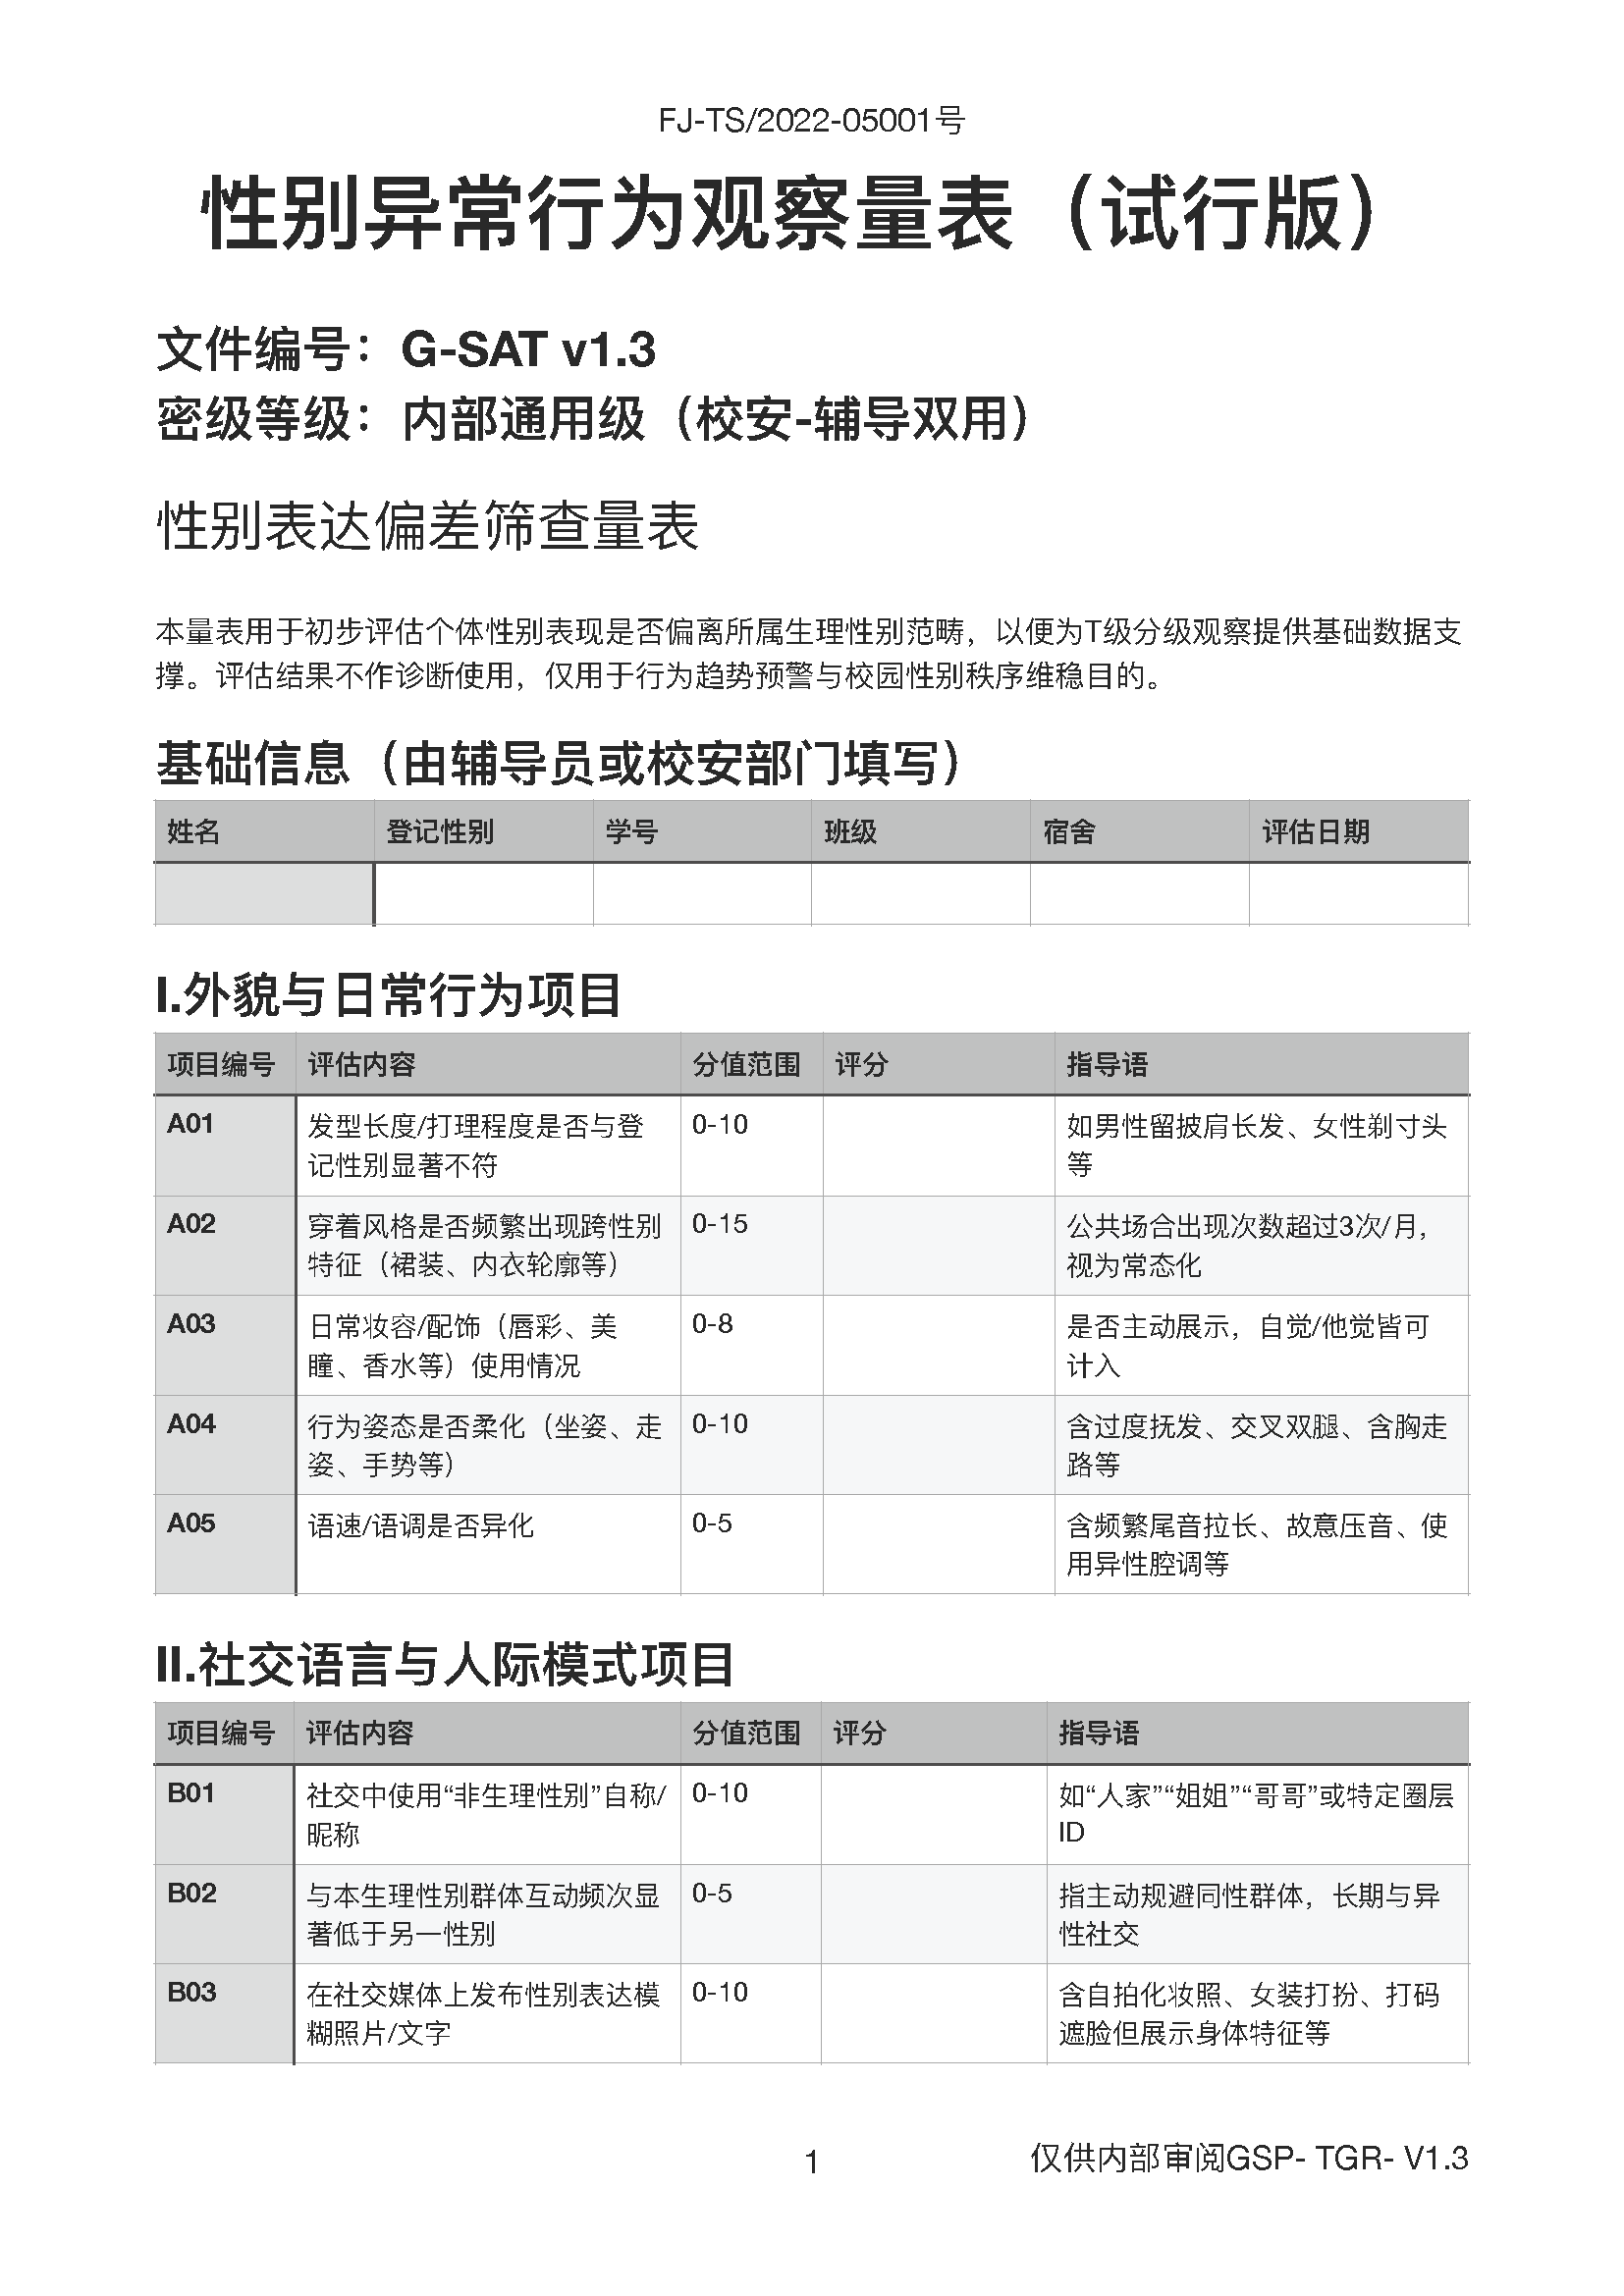
\includegraphics[scale=0.6]{./附件1正文_页面_1.png}
	
	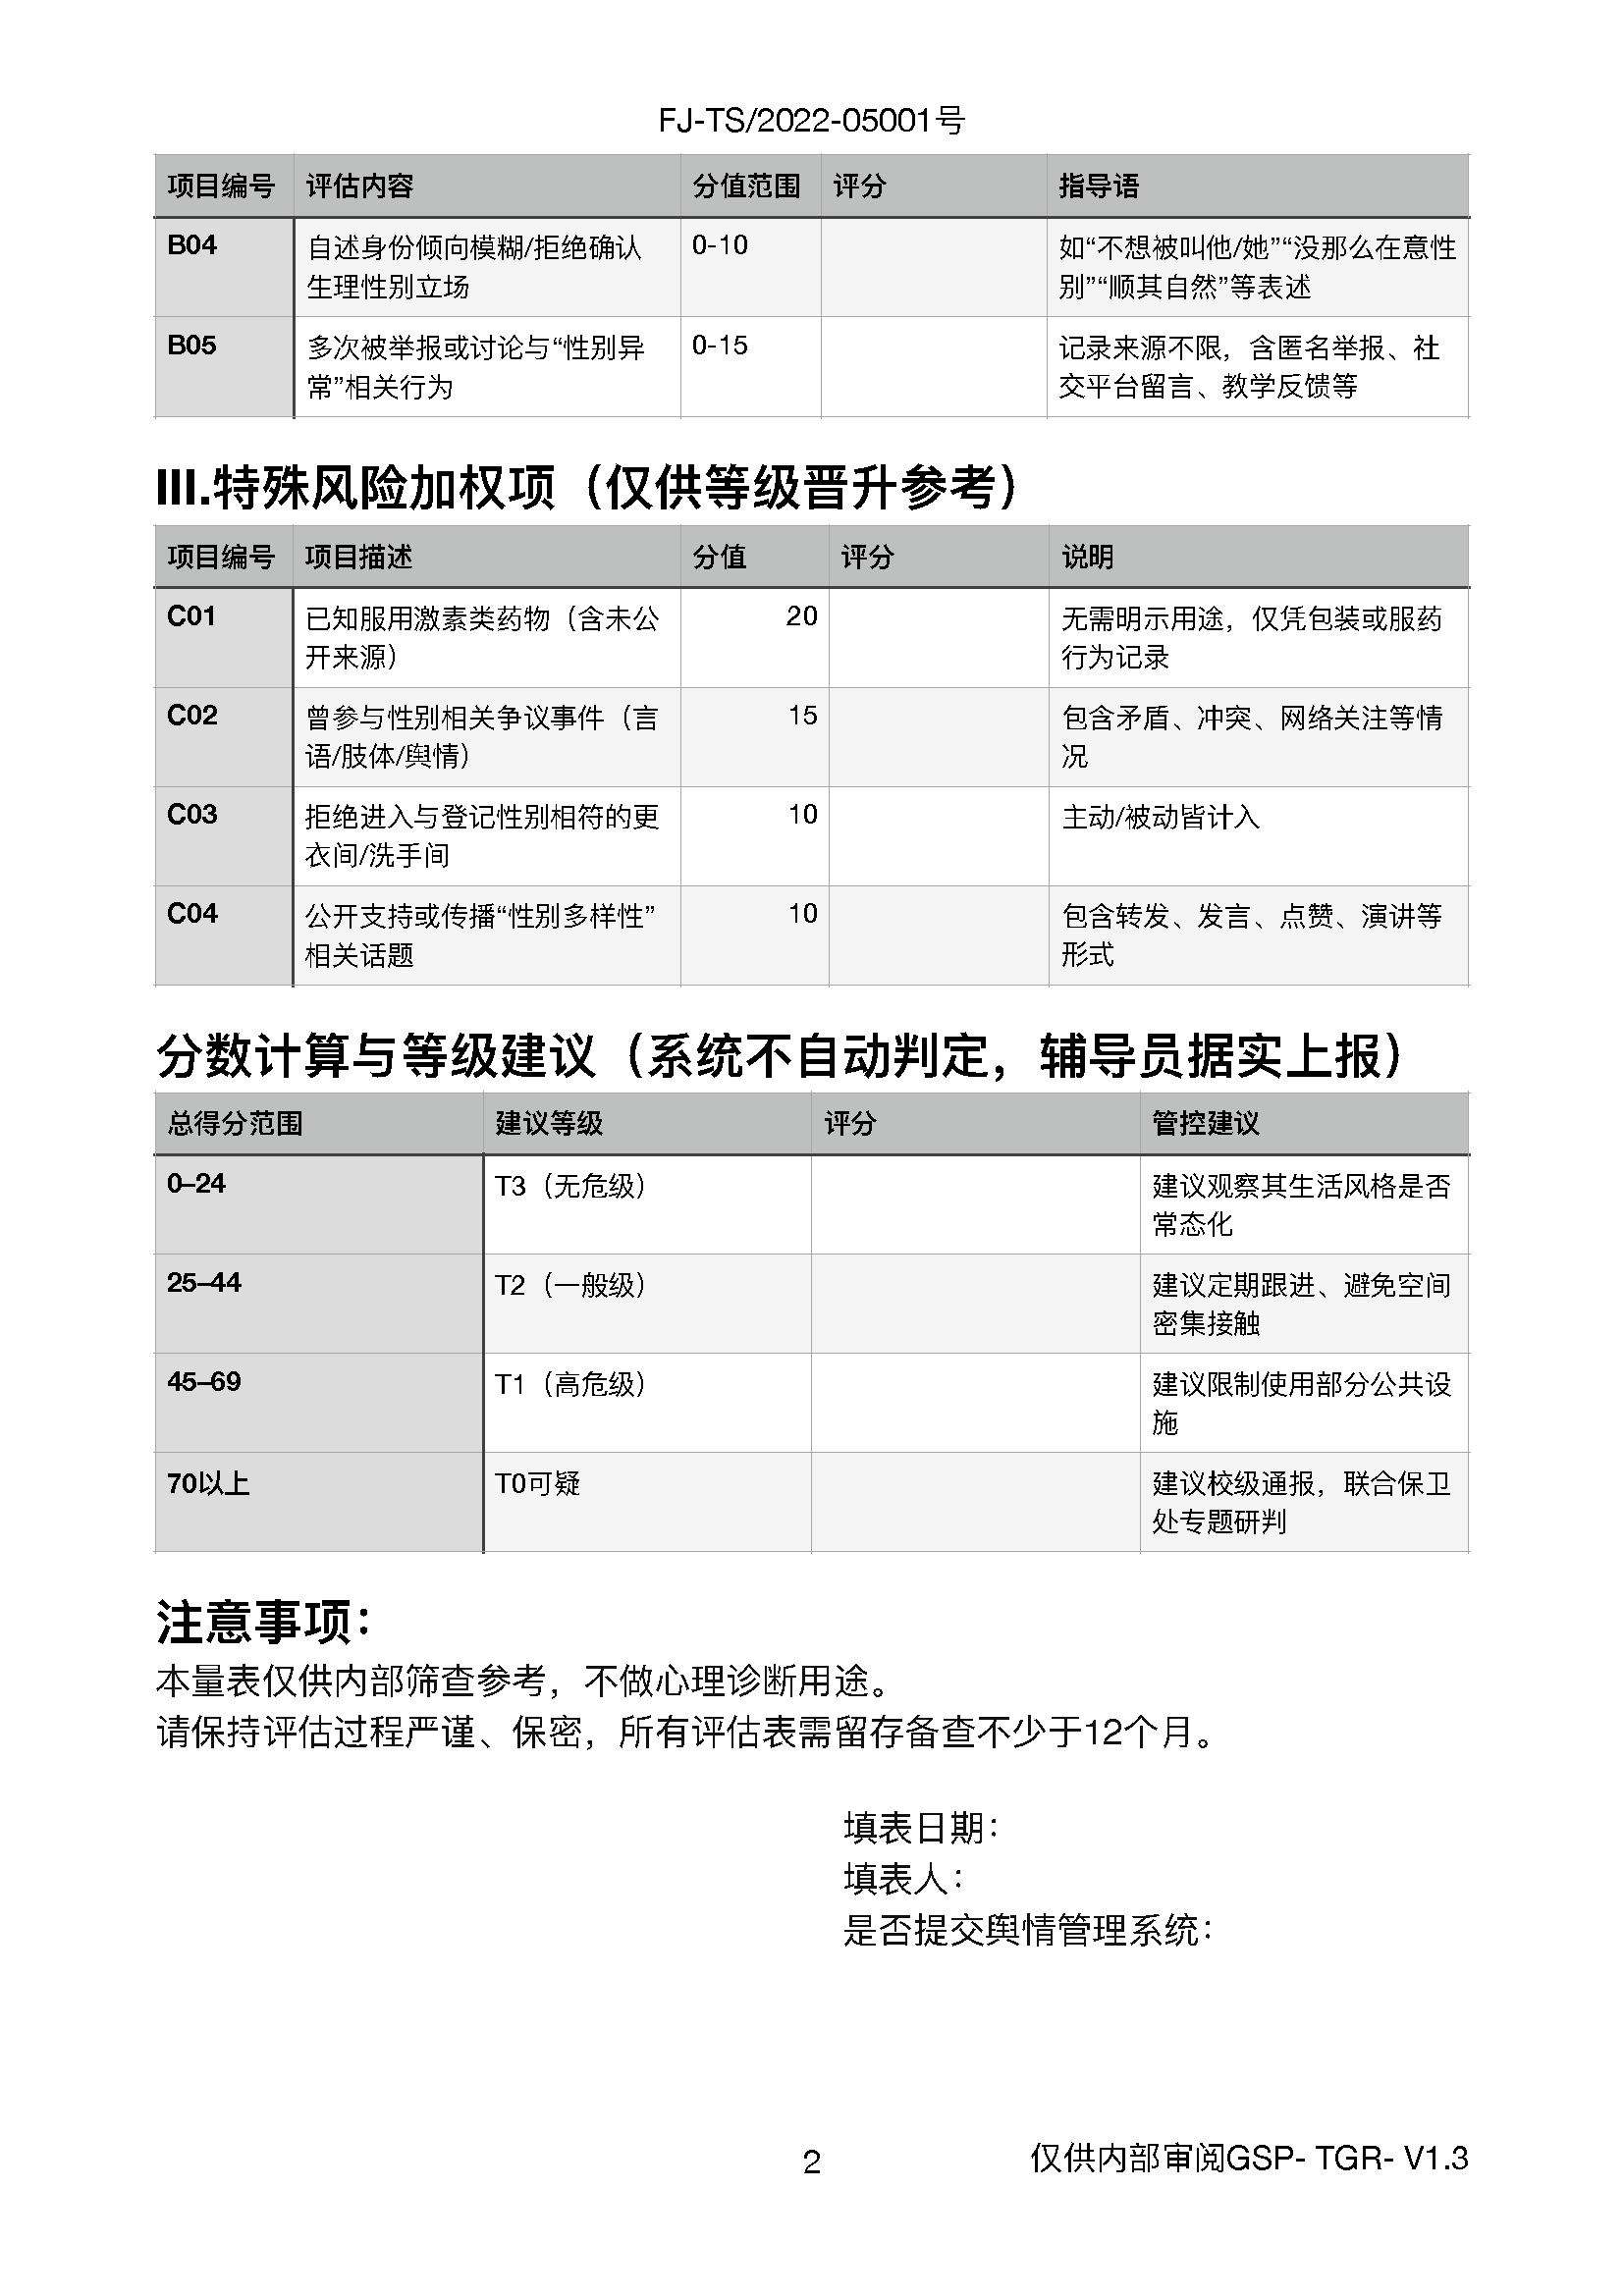
\includegraphics[scale=0.6]{./附件1正文_页面_2.png}
	
	\section*{附件2. 校内举报信息汇编}
	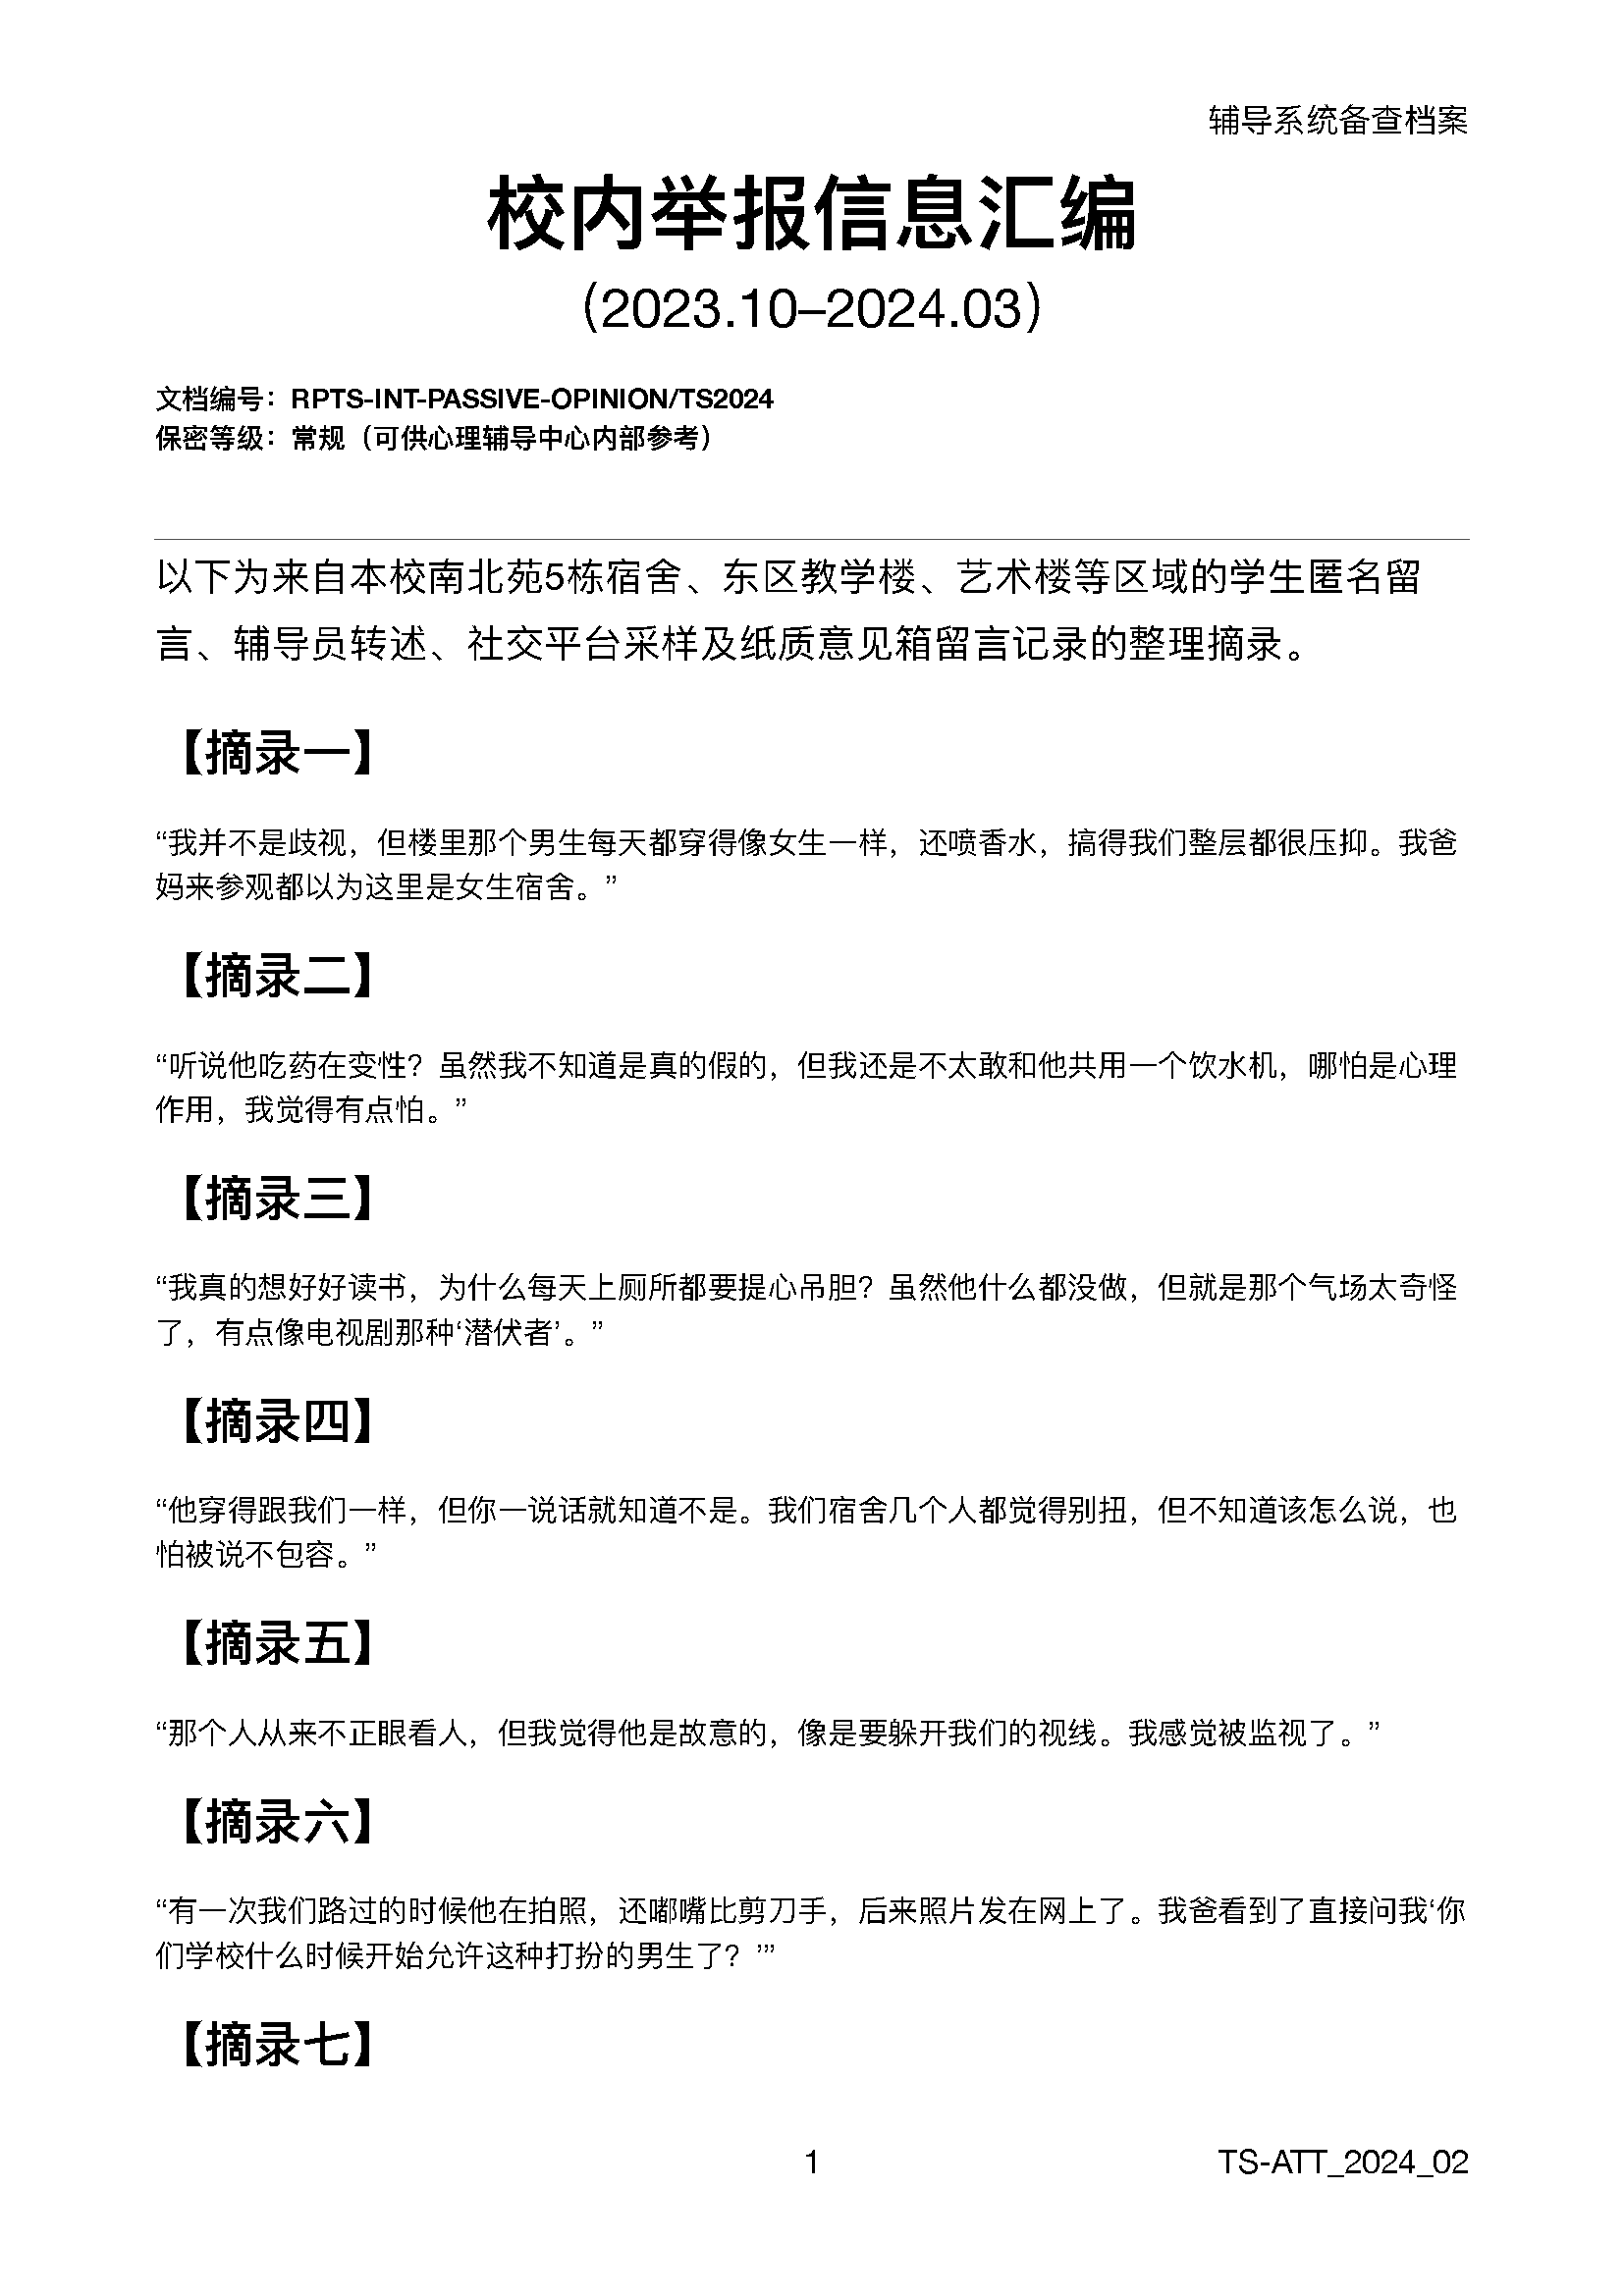
\includegraphics[scale=0.6]{./附件2正文_页面_1.png}
	
	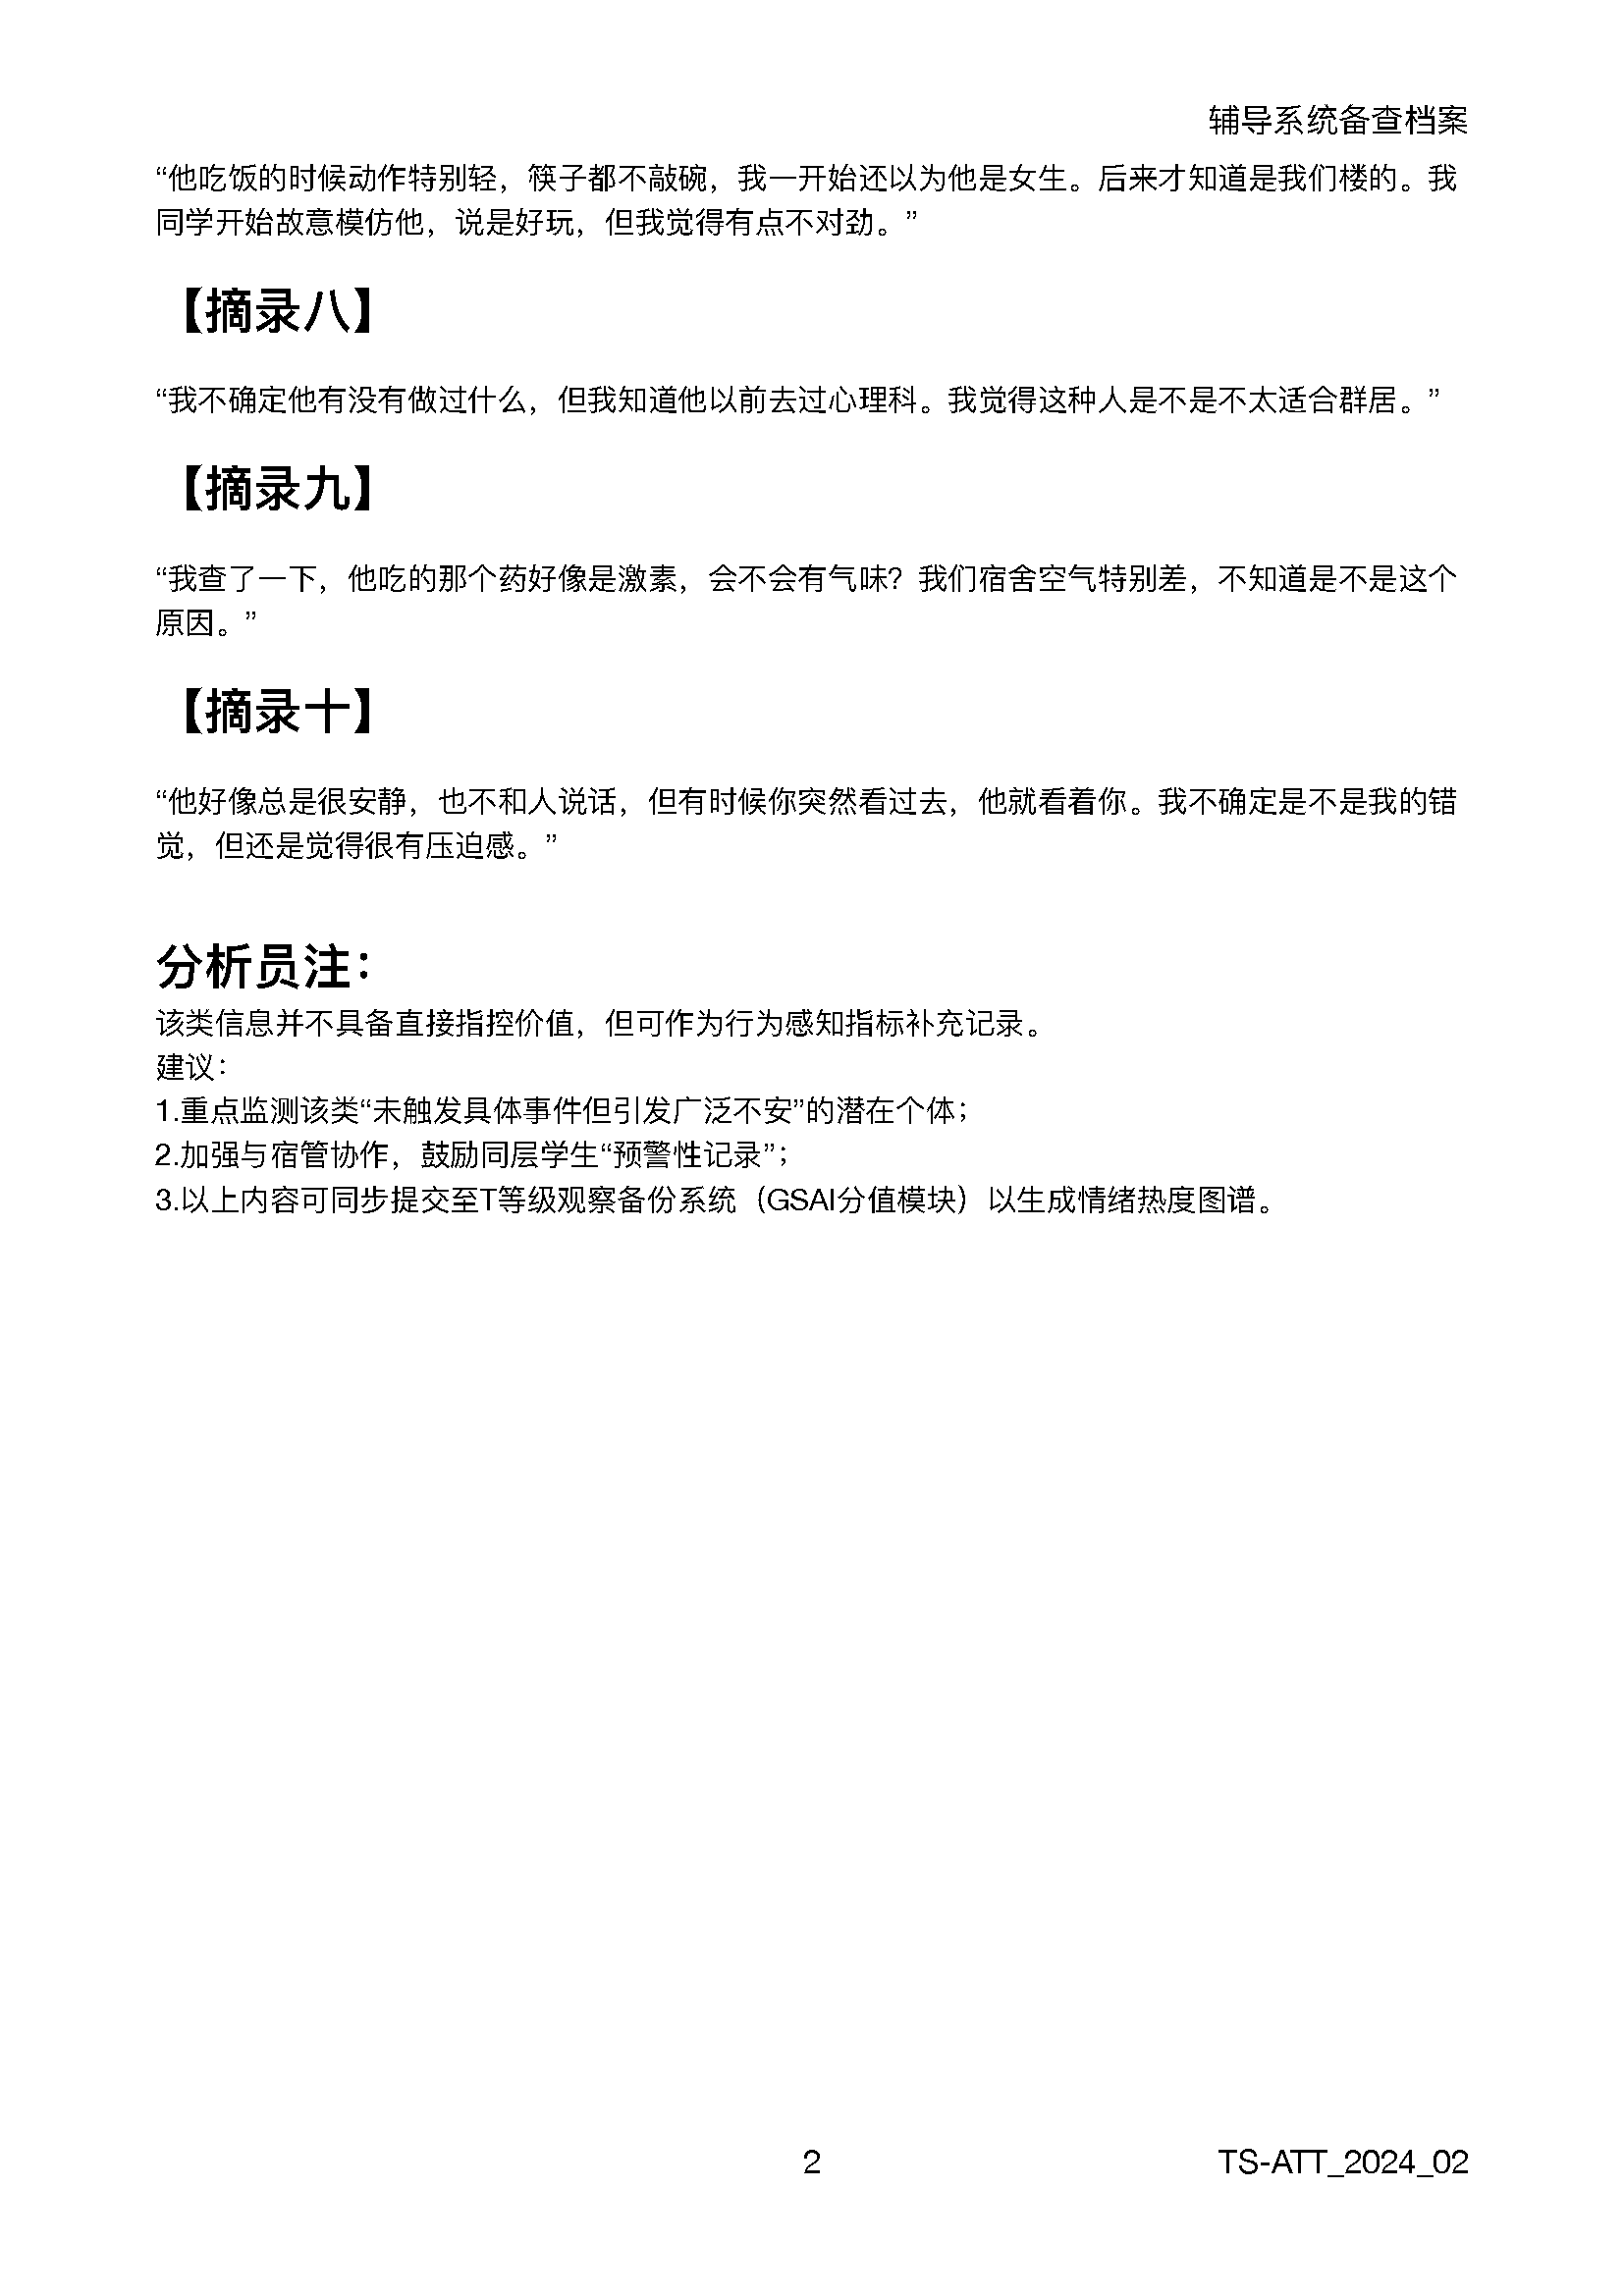
\includegraphics[scale=0.6]{./附件2正文_页面_2.png}
	
	\section*{附件3.1 送检标本检测报告单}
	\label{附件3.1}
	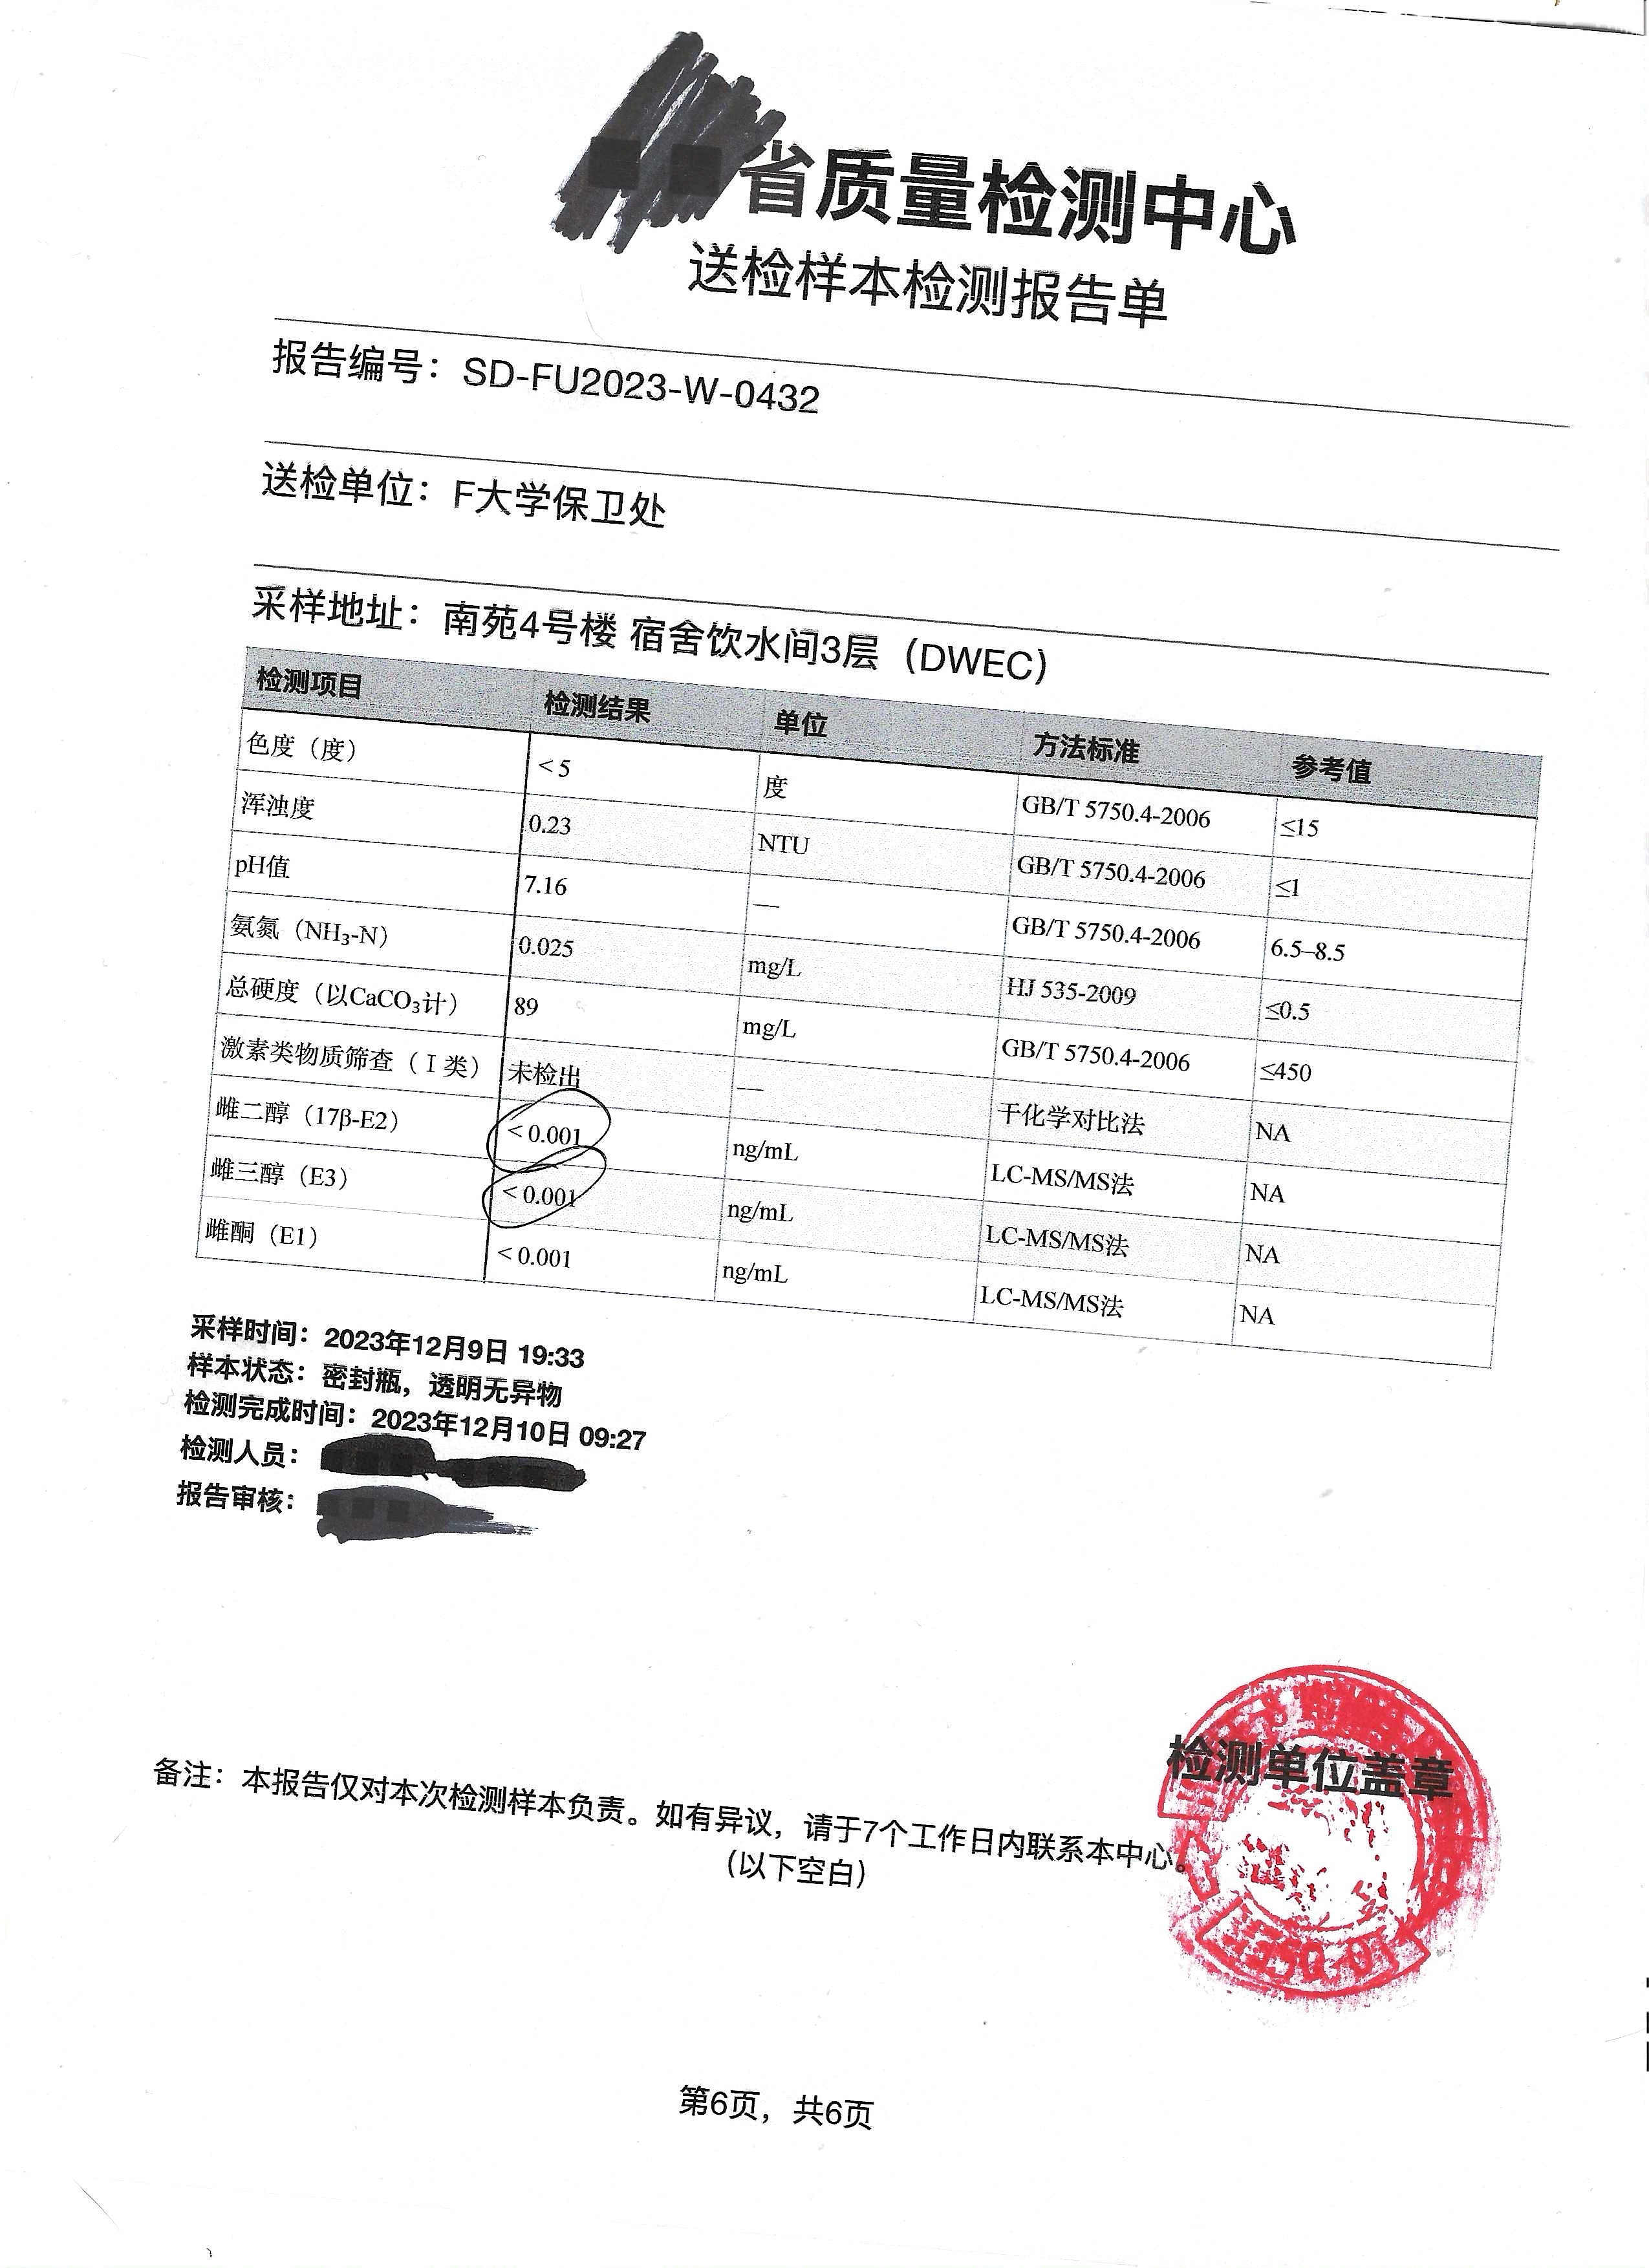
\includegraphics[scale=0.6]{./附件3.1.png}
	
	\section*{附件3.2 补佳乐处方凭证(T2-078个体)}
	\label{附件3.2}
	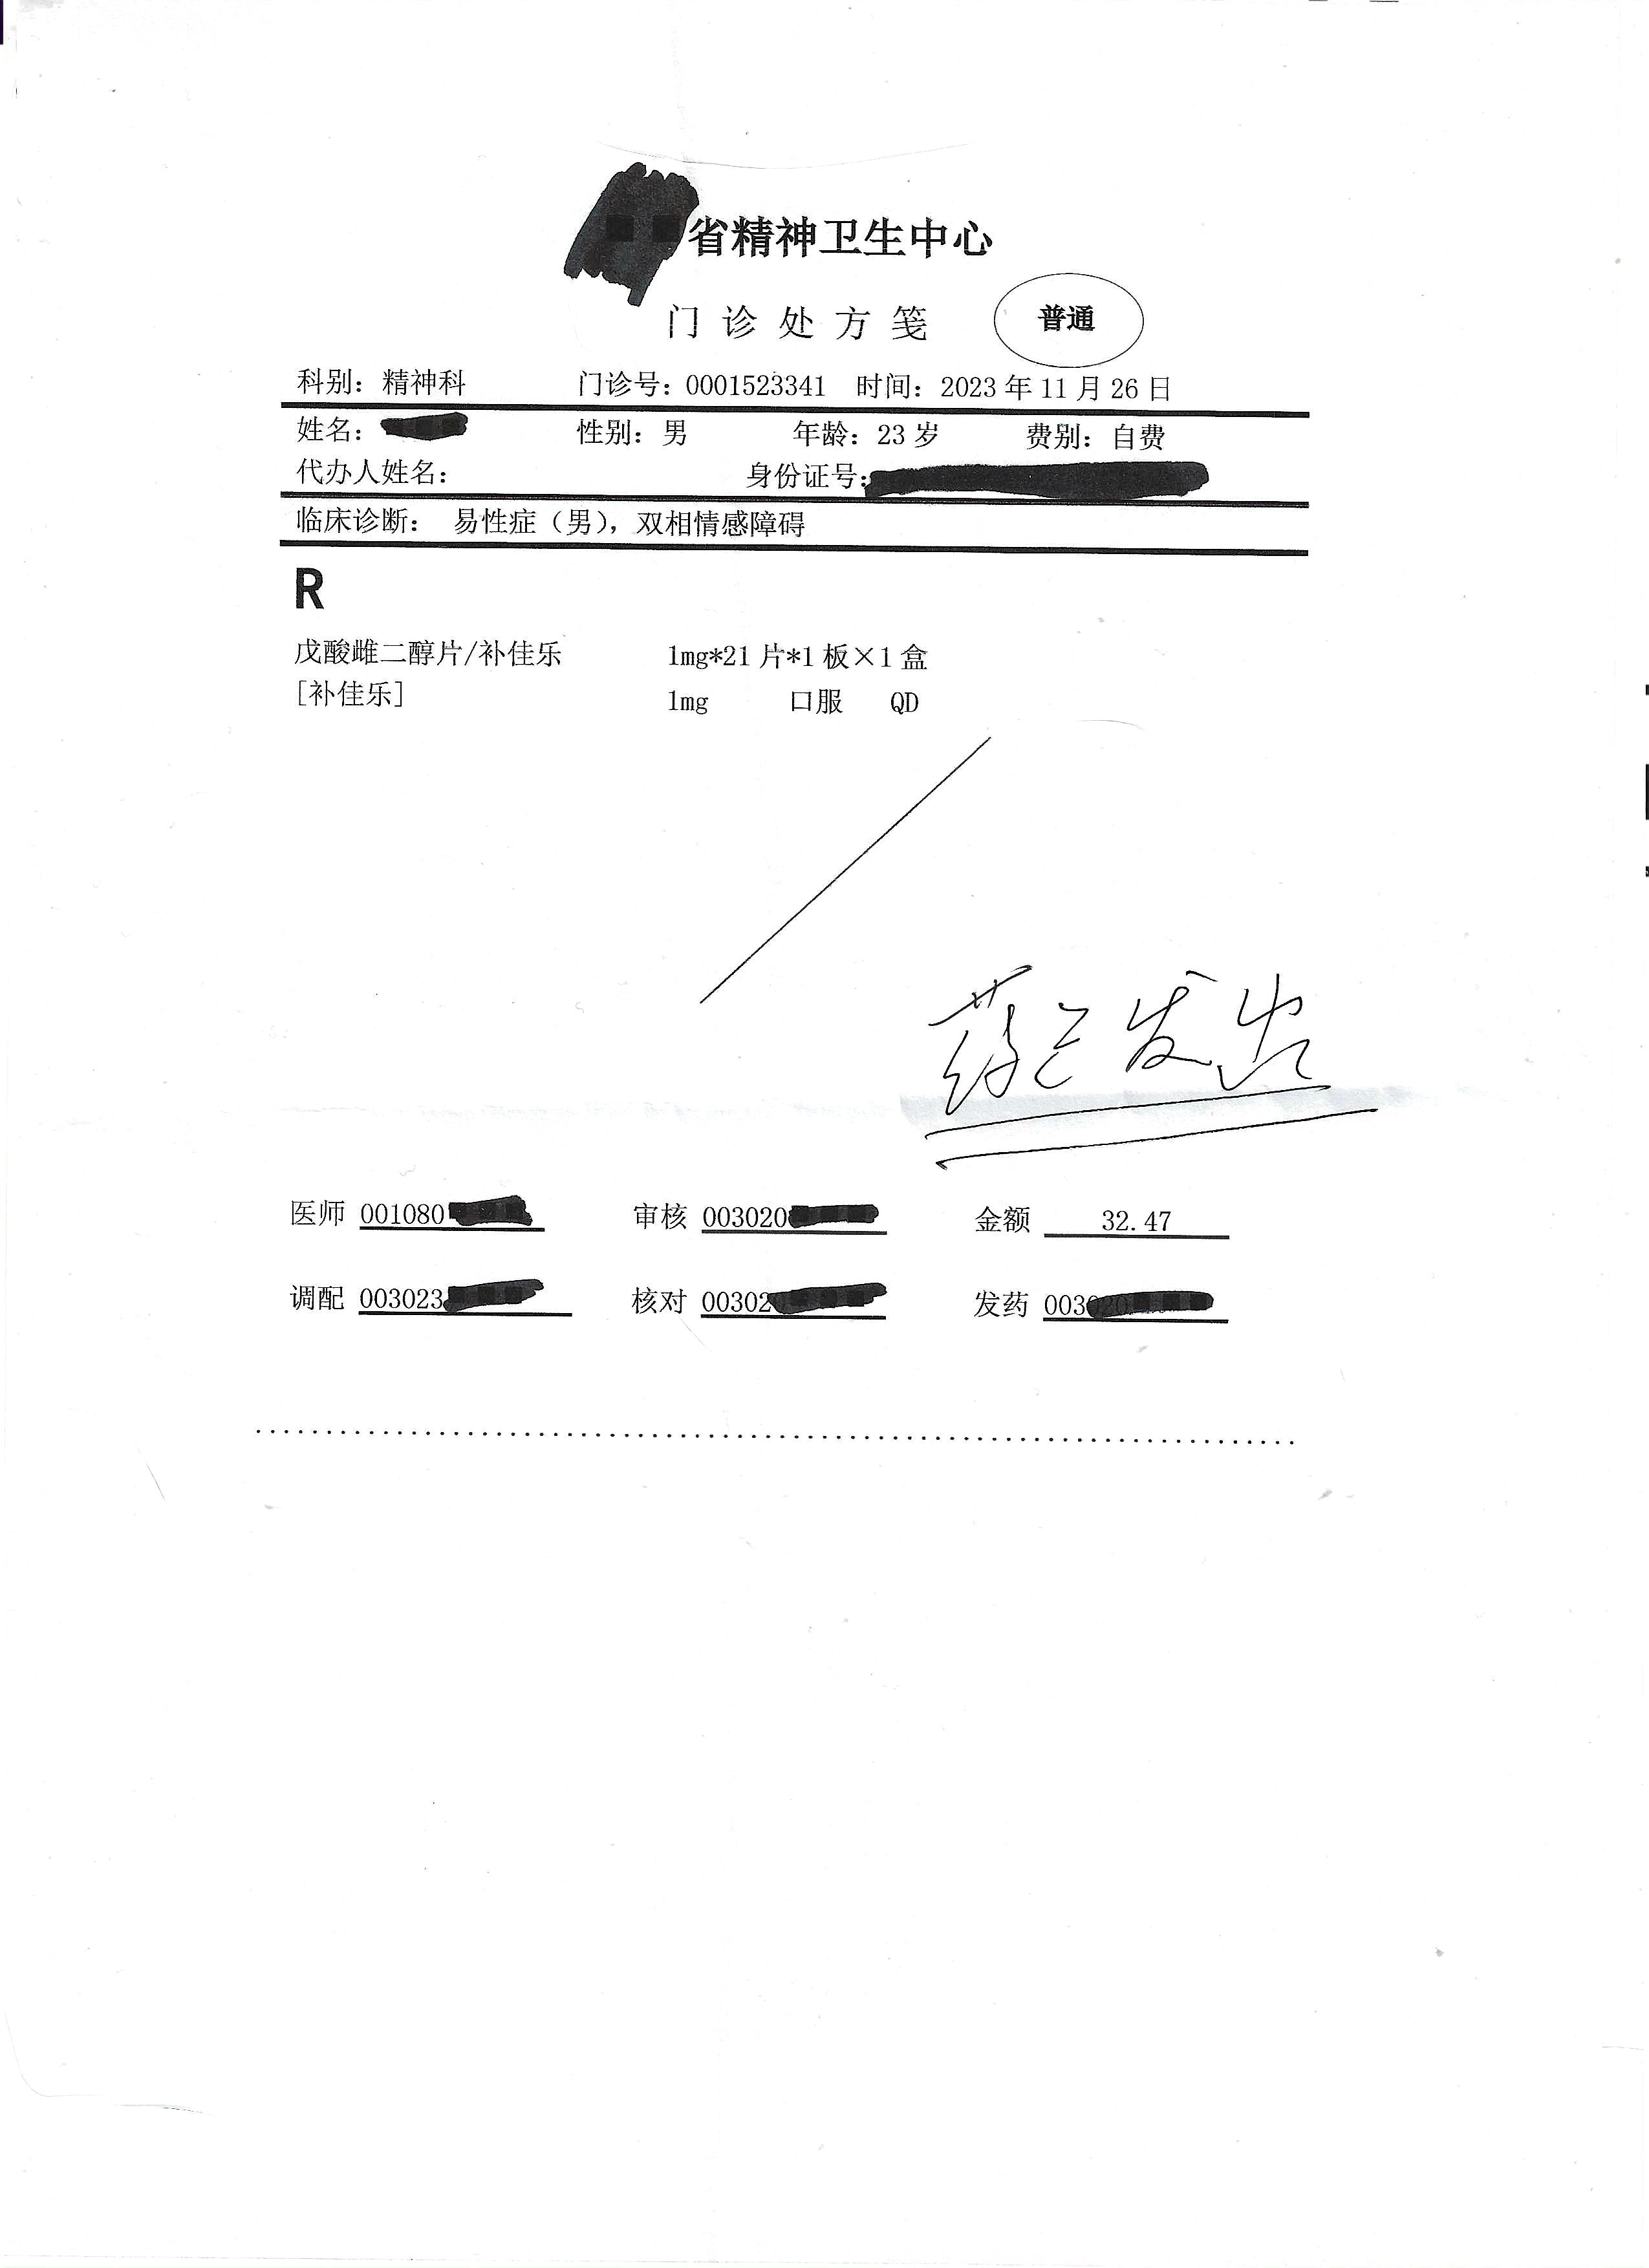
\includegraphics[scale=0.6]{./附件3.2.png}
	
	\section*{附件4. T3-112个体公共活动影像社交记录截图}
	\label{附件4}
	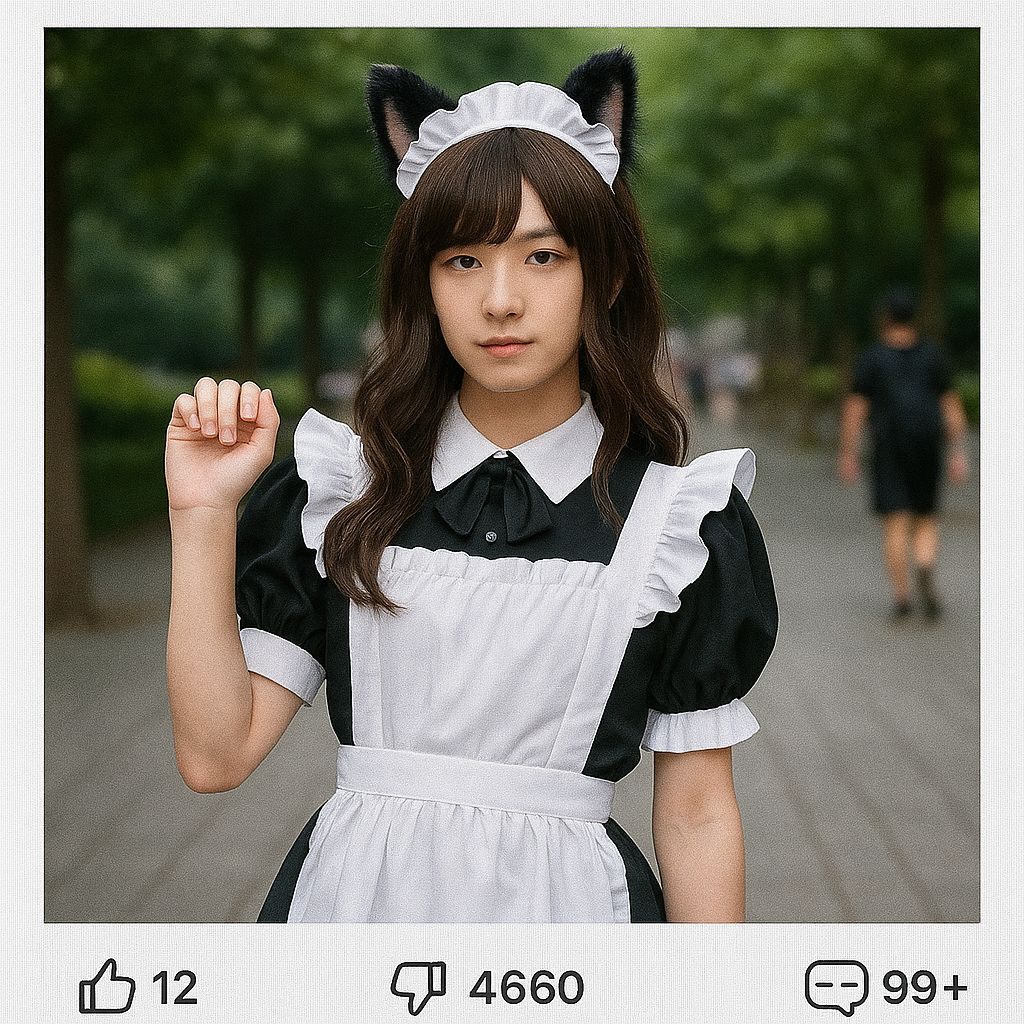
\includegraphics[scale=0.3]{./附件4.png}
	
	\newpage
	\section*{附件5.1 T0-001个体的医疗器械说明文档}
	\label{附件5.1}
	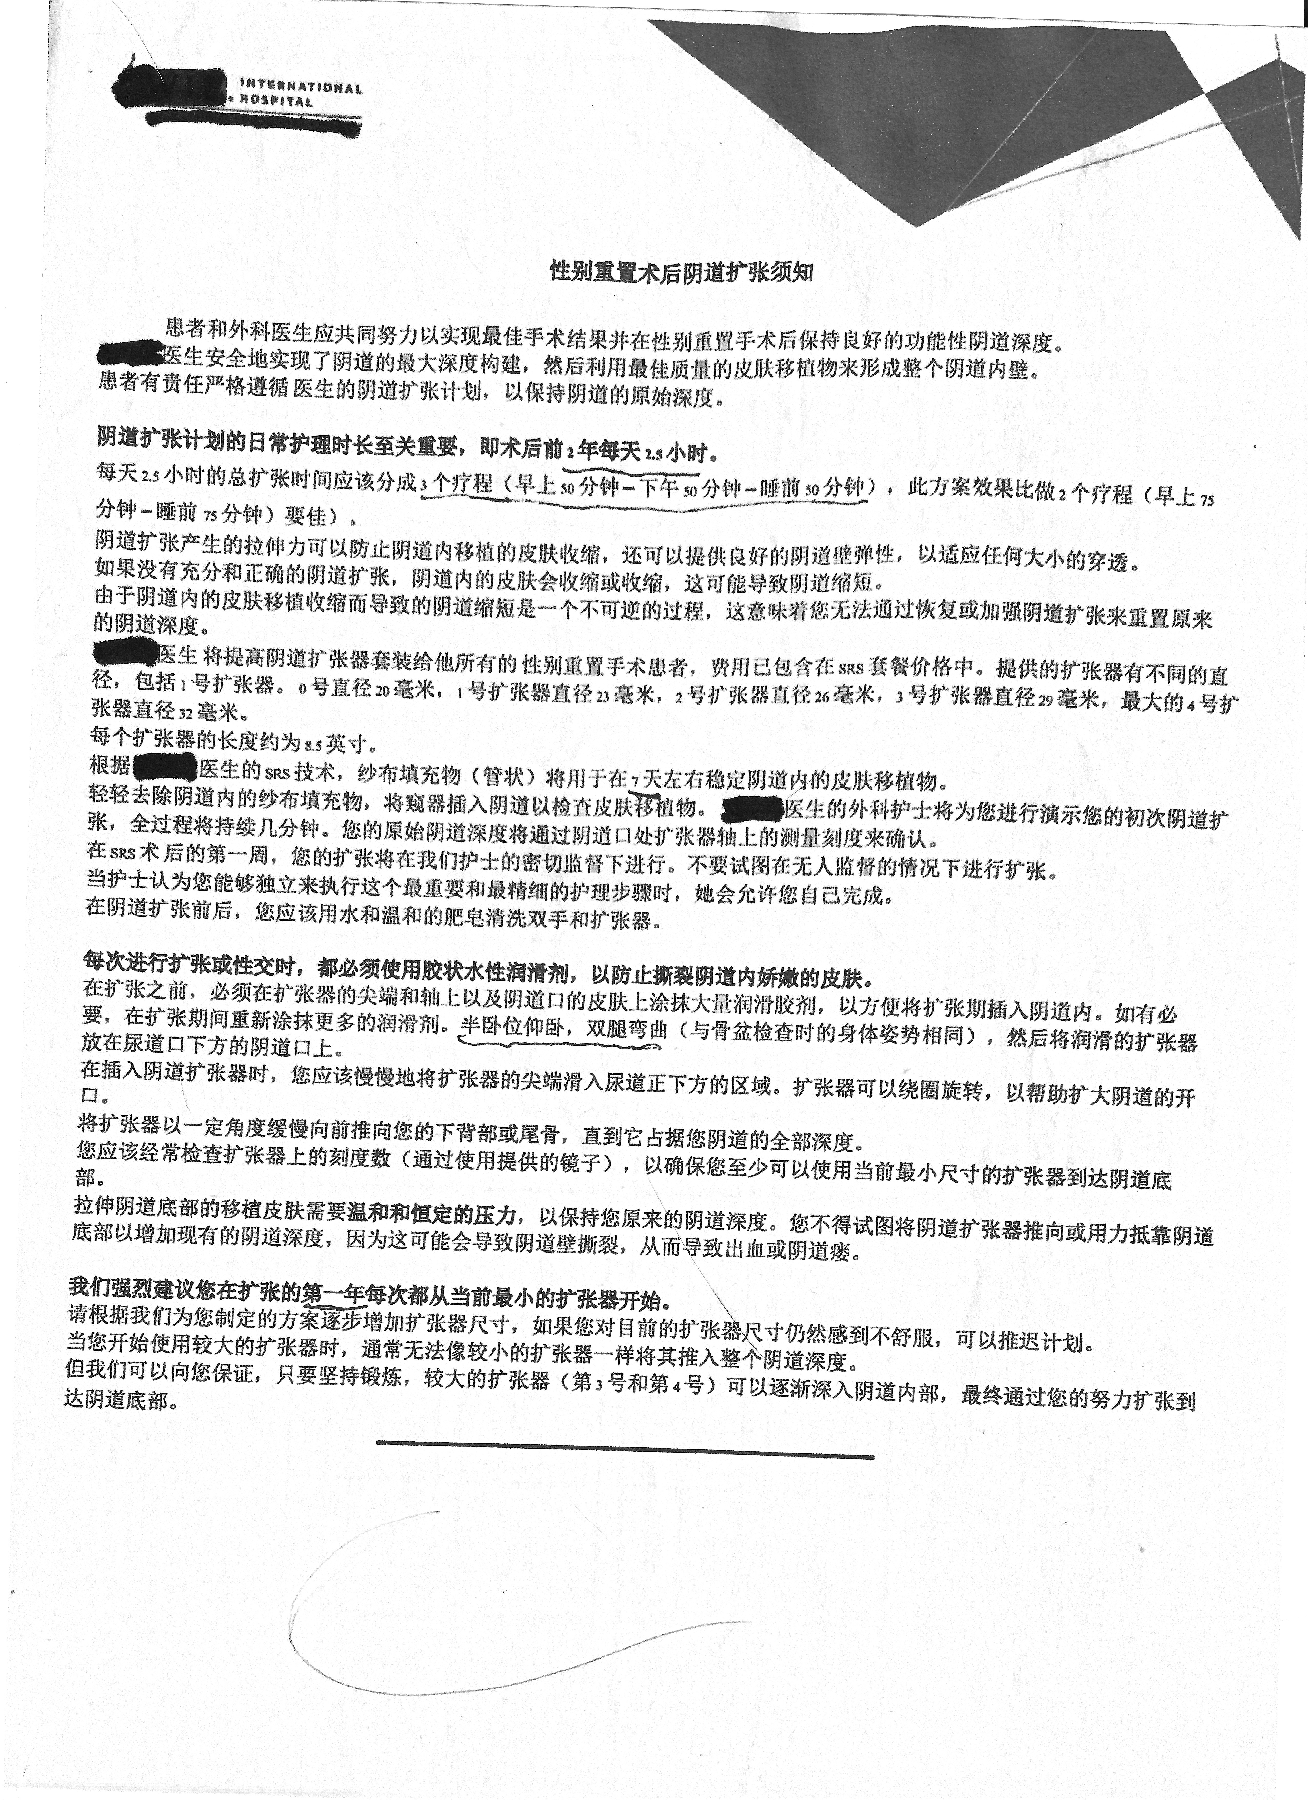
\includegraphics[scale=0.4]{./附件5.1.1.png}
	
	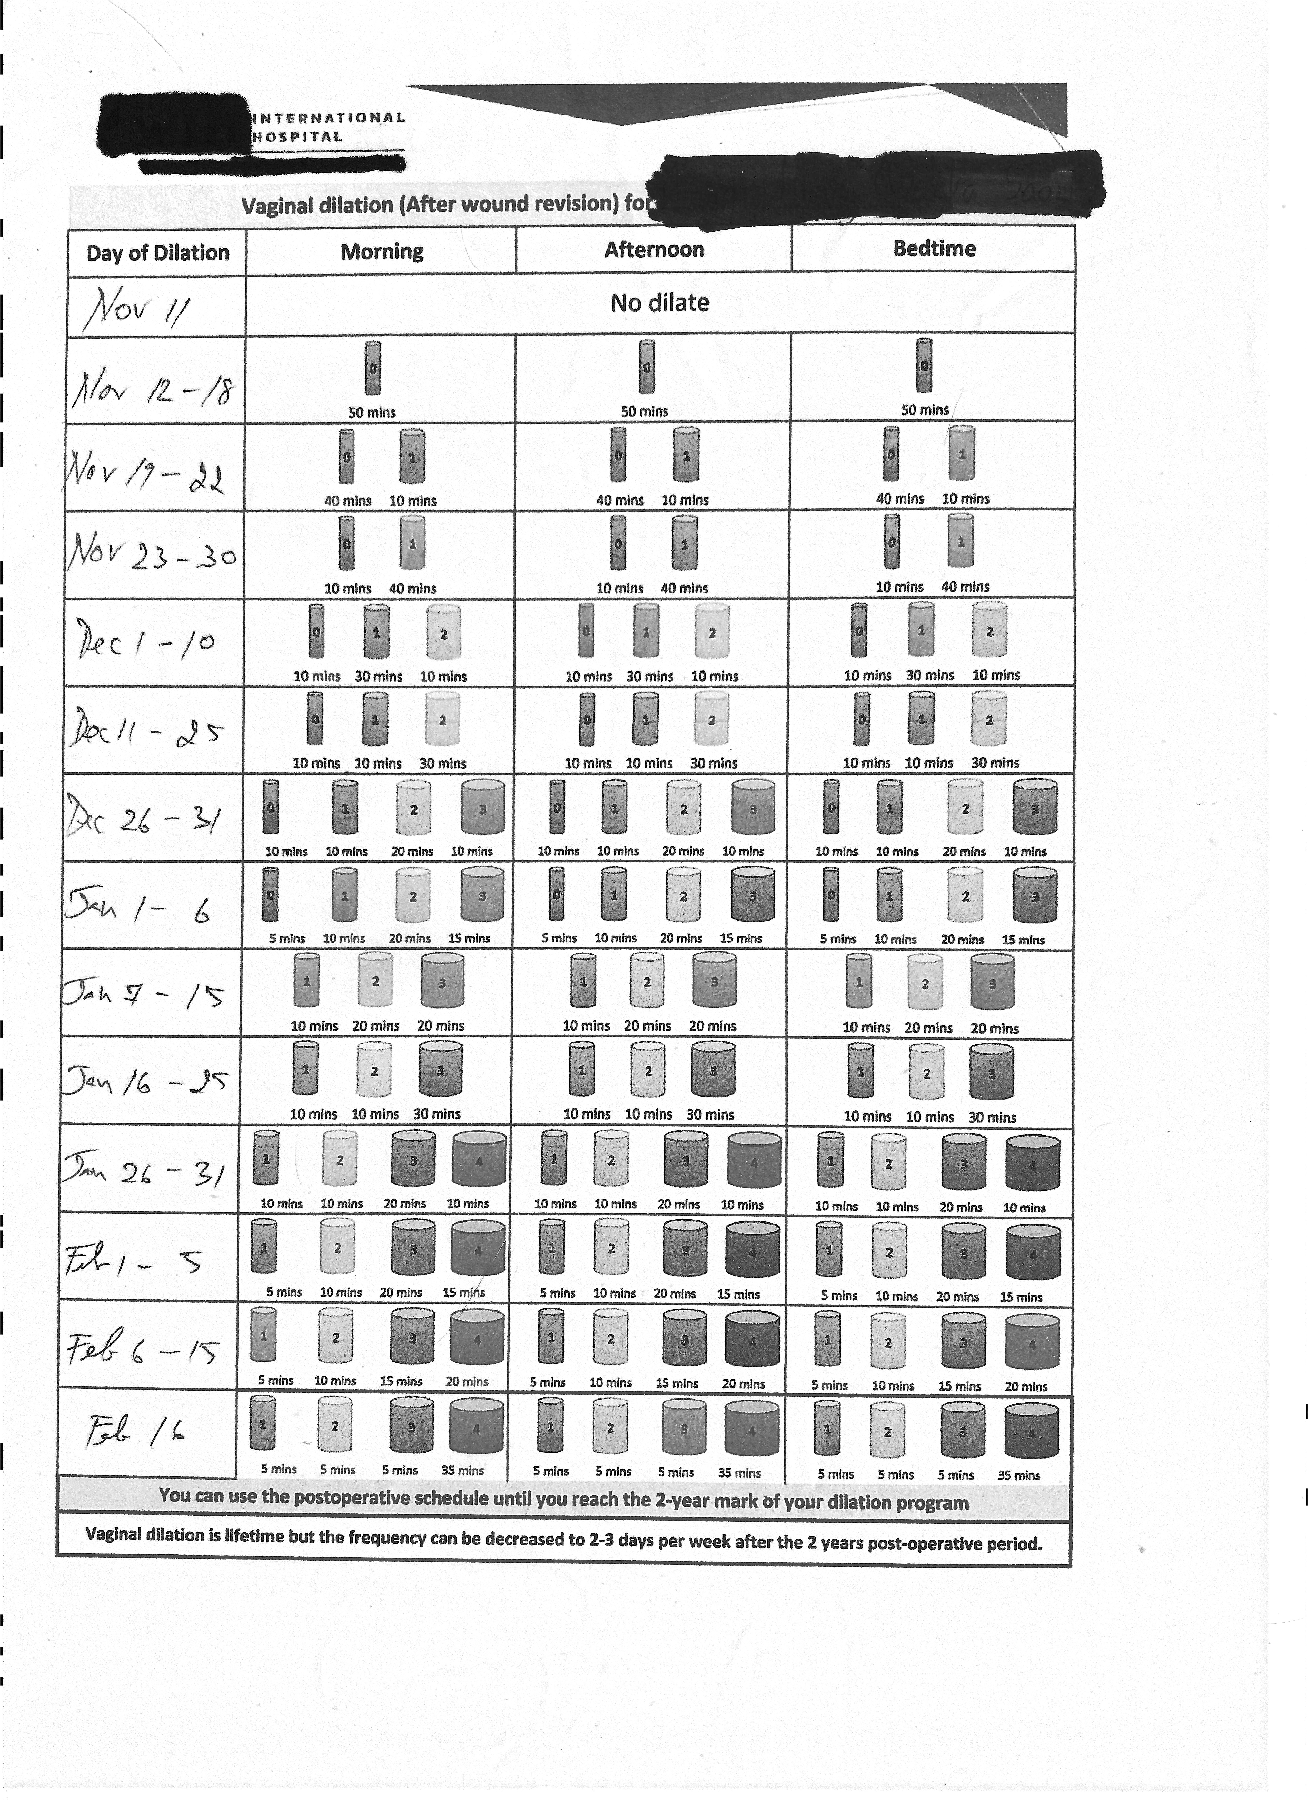
\includegraphics[scale=0.4]{./附件5.1.2.png}
	
	\section*{附件5.2 T0-001个体的司法鉴定意见书}
	\label{附件5.2}
	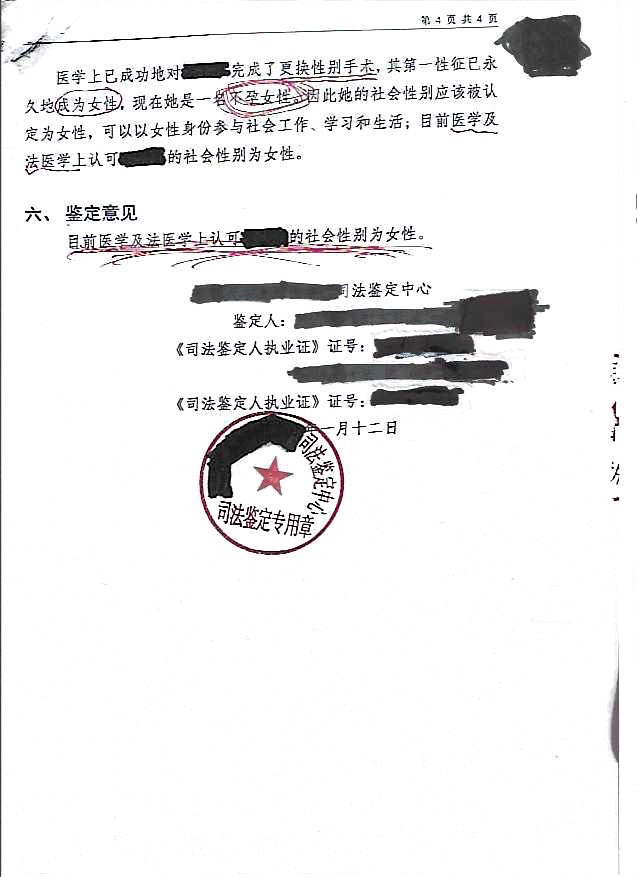
\includegraphics[scale=0.6]{./附件5.2.png}
	
	\newpage
	\section*{附件X 个体编号T1-031的检讨书}
	
	\noindent 尊敬的各位领导,各位老师,亲爱的同学和舍友们:
	
	你们好吗?我在此写下了这份检查,因为我深刻意识到,自己的所作所为,是多么的幼稚、愚蠢和傲慢。
	
	我深刻地认识到,我作为一个被登记在案的T等级个体,我是绝对没有想做什么就做什么的自由的,我的一切言行也好,举止也罢,都必须被牢牢地关在制度的笼子里。老话说,没有规矩,不成方圆。我今天能打破规矩,明天就能打破天空。学校为了我们学生的身心健康着想而订立的规则,而我,作为一个登记在册、应受管理的T等级个体,居然妄想取得我不敢奢求的自由,这是多么的无法无天!为此,我深深忏悔。
	
	我本应铭刻在心地知道,作为一个被登记在案的T等级个体,我本应限制进入任何的公共场所,我天生就有顾忌别的同学身心健康的责任和义务,我的生理反应也好,我的日常生活也好,必须建立在保持绝大多数性别正常同学的基础和前提下而进行。而我居然胆大包天,仅仅是因为内急,就无法跑到三公里外的T级个体指定的卫生间去解决,反而像无头苍蝇一样扎进了充满正能量和无限青春活力的正常同学使用的卫生间。我的所作所为,简直是不把学校的规章制度和管理制度放在眼里,如此无法无天的行为,本应受到无限的惩罚和谴责。为此,我深深忏悔。
	
	我本应清楚并清晰地知道,我作为一个登记在案的T等级个体,我本就不应该将自己的肮脏药物带入任何正常同学能看得见的地方。我生来就是传播犯罪与乱伦的病原体,我的日常用药,则更应该被好好保管,严格存放。而我居然疏忽大意,将药物与其他正常同学所处的时空混为一谈,就像在一张纯净的白纸上涂满了暗黑的恐惧一样。我本应该尽到严格保管的责任和义务,而且却任由性别正常的同学翻动我的柜子和书包,接触到了他们本应永远接触不到的严重的致病物质。我的所作所为,简直与故意杀人和蓄意投毒无异,就应该受到道德的惩罚与制度的灭杀。为此,我深深忏悔。
	
	我本应该严格并坚定地知道,我作为一个登记在册的T等级个体,我本应该和其他非典型性别个体保持距离,并应时时刻刻借着制度下对我们留有的恩惠和空间,过好不影响别人的生活。而我居然,极其残忍和残酷,居然对同校的疑似有非典型性别倾向的同学进行了鼓励、致意和尊重。这就像本应翱翔天空的鱼儿和潜游水底的猎鹰,我所鼓励的,是犯罪,是罪恶,是恶灵,是灵柩。是无可原谅的滑坡式从山顶走向深渊滚落巨石而不可挽回的。一颗纯真善良的心灵本应受到醺醺善诱而不会收到乳香的炙烤以及各种各样来自不同地方世界有害气体与不存在的有害气体物质环境。为此我深深忏悔。
	
	我将在余下的时间里封存我的声音缝合我的表达暂停我的存在我将消隐于走廊尽头避让于水声前方隐匿于同学眼神投来的路径以外。若能这样我或许还能部分恢复一个正常人应有的秩序价值为此我深深忏悔。
	
	在最后,请允许卑微的我,向学校、向教职工老师们、向本应遵守的制度献上最后的敬意。
	
	愿光荣归于学校及师及制度,起初如何,今日亦然,直到永远。
	
	因权、及利、及制度之名。
	
	为此,我深深忏悔。
	
	为此,我再次忏悔。
	
	为此,我最终忏悔。
	
	\vspace{6in}
	
	\begin{flushright}
		个体编号:T1-031\\
		签字人(已退学):████\\
		时间:2024年4月1日
	\end{flushright}
	
	\chapter*{总结声明与免责条款}
	
	你读到了这里,非常好。你已经完成了一份调查报告的全文阅读。你是不是也感受到了一种舒适的逻辑闭环感?有标准,有流程,有系统,有结论,一切都安排得滴水不漏。
	
	只是,我们真的在谈论“秩序”吗?
	还是,只是用“秩序”来清理掉你不愿意看到的“例外”?
	
	你真的在读一个恶意制造的世界吗?
	还是你其实,早就生活在这里了。
	
	\begin{center}
		\textcolor{red}{{\Large \textbf{以上报告纯属虚构,如有雷同,你该反思一下你自己了。}}}
	\end{center}
	\vspace{3in}
	\begin{flushright}
		——Min Francis Liu\\
		——George Peter Terra\\
		——Gekka Saori\\
		——Mc'Flurry Felis\\
	\end{flushright}
	{\Large 文本注销编号:TGR-404-NULL\\
		请将本页焚毁,撒向风中。}
	
	
	
	
	
\end{document}